% !TeX program = xelatex
\documentclass[12pt,a4paper,oneside]{report}

% ==================== GÓI CƠ BẢN ====================
\usepackage[a4paper,top=2.5cm,bottom=2.5cm,left=3cm,right=2cm]{geometry}
\usepackage{fontspec}
\usepackage{polyglossia}
\setdefaultlanguage{vietnamese}
\setotherlanguage{english}
\setmainfont{Times New Roman}
\setsansfont{Times New Roman}
\setmonofont{Courier New}

\usepackage{setspace}
\onehalfspacing
\setlength{\parindent}{1.25cm}
\setlength{\parskip}{0.25em}

\usepackage{graphicx}
\graphicspath{{figures/}}
\usepackage{float}
\usepackage{subcaption}
\usepackage{booktabs}
\usepackage{tabularx}
\usepackage{longtable}
\usepackage{array}
\usepackage{multirow}
\usepackage{makecell}
\usepackage{enumitem}
\usepackage{amsmath,amssymb}
\usepackage{siunitx}
\usepackage{xcolor}
\usepackage{listings}
\usepackage{caption}
\usepackage{chngcntr}
\usepackage{titlesec}
\usepackage{tikz}
\usetikzlibrary{arrows.meta,positioning,shapes.geometric}
% Đặt sau titlesec để cả đoạn đầu tiên sau tiêu đề mục cũng được thụt đầu dòng.
\usepackage{indentfirst}
\usepackage{fancyhdr}
\usepackage{hyperref}
\usepackage[backend=biber,style=ieee,sorting=none]{biblatex}
\addbibresource{references.bib}

% ==================== THIẾT LẬP TRÌNH BÀY ====================
\definecolor{hcmusblue}{RGB}{23,70,115}
\hypersetup{
    colorlinks=true,
    linkcolor=hcmusblue,
    citecolor=hcmusblue,
    urlcolor=hcmusblue,
    pdftitle={Báo cáo cuối kỳ - Hệ thống Hỏi đáp Y tế tiếng Việt},
    pdfauthor={Nhóm 12}
}

\titleformat{\chapter}[hang]
  {\bfseries\Large}
  {Chương \thechapter.}{0.6em}{}
\titlespacing*{\chapter}{0pt}{-20pt}{18pt}
\titleformat{\section}{\bfseries\large}{\thesection}{0.6em}{}
\titleformat{\subsection}{\bfseries\normalsize}{\thesubsection}{0.6em}{}
% Không dùng dấu *: giữ thụt đầu dòng cho đoạn văn ngay sau section/subsection.
\titlespacing{\section}{0pt}{3.5ex plus 1ex minus .2ex}{2.3ex plus .2ex}
\titlespacing{\subsection}{0pt}{3.25ex plus 1ex minus .2ex}{1.5ex plus .2ex}

\captionsetup{font=small,labelfont=bf,labelsep=period}
\counterwithin{figure}{chapter}
\counterwithin{table}{chapter}
\counterwithin{equation}{chapter}

\pagestyle{fancy}
\fancyhf{}
\fancyhead[L]{\small Báo cáo cuối kỳ - Nhóm 12}
\fancyhead[R]{\small \leftmark}
\fancyfoot[C]{\thepage}
\renewcommand{\headrulewidth}{0.4pt}

\lstset{
  basicstyle=\ttfamily\small,
  breaklines=true,
  frame=single,
  numbers=left,
  numberstyle=\tiny,
  showstringspaces=false,
  tabsize=4,
  captionpos=b
}

% Cột bảng tiện dụng
\newcolumntype{Y}{>{\raggedright\arraybackslash}X}
\newcommand{\placeholder}[1]{\textcolor{gray}{\textit{[#1]}}}
\tikzset{
  process/.style={draw=hcmusblue, rounded corners=2pt, fill=hcmusblue!7,
    align=center, minimum height=1.15cm, text width=3.15cm, inner sep=5pt},
  decision/.style={diamond, draw=hcmusblue, fill=hcmusblue!7,
    align=center, aspect=2.1, inner sep=2pt, text width=2.2cm},
  flow/.style={-{Latex[length=2.5mm]}, thick, draw=hcmusblue}
}

% ==================== THÔNG TIN BÁO CÁO ====================
\newcommand{\university}{ĐẠI HỌC QUỐC GIA TP. HỒ CHÍ MINH}
\newcommand{\school}{TRƯỜNG ĐẠI HỌC KHOA HỌC TỰ NHIÊN}
\newcommand{\faculty}{KHOA CÔNG NGHỆ THÔNG TIN}
\newcommand{\reporttitle}{BÁO CÁO CUỐI KỲ}
\newcommand{\projecttitle}{HỆ THỐNG HỎI - ĐÁP Y TẾ TIẾNG VIỆT}
\newcommand{\coursename}{Nhập môn học máy}
\newcommand{\coursecode}{CSC14005}
\newcommand{\classcode}{CQ2023/24}
\newcommand{\semester}{Học kỳ 2 - 2025/2026}
\newcommand{\lecturer}{Bùi Tiến Lên}
\newcommand{\groupname}{Nhóm 12}

\begin{document}

% ==================== TRANG BÌA ====================
\begin{titlepage}
\begin{center}
    {\bfseries\large \university\\[0.25cm]}
    {\bfseries\large \school\\[0.25cm]}
    {\bfseries\large \faculty}

    \vspace{1.2cm}
    \IfFileExists{figures/logo-hcmus.jpg}{
        \includegraphics[width=5.2cm]{logo-hcmus.jpg}
    }{
        \fbox{\parbox[c][5cm][c]{5cm}{\centering Logo\\HCMUS}}
    }

    \vspace{1.2cm}
    {\bfseries\Large \reporttitle\\[0.45cm]}
    {\bfseries\LARGE \projecttitle}

    \vspace{1.2cm}
    \begin{tabular}{@{}ll@{}}
        \textbf{Môn học:} & \coursename\\
        \textbf{Mã môn học:} & \coursecode\\
        \textbf{Lớp:} & \classcode\\
        \textbf{Học kỳ:} & \semester\\[0.3cm]
        \textbf{Giảng viên hướng dẫn:} & \lecturer
    \end{tabular}

    \vspace{0.8cm}
    \textbf{Nhóm sinh viên thực hiện:}\\[0.25cm]
    \begin{tabular}{@{}lll@{}}
        & Nguyễn Nhật Lân & 23120289\\
        & Y Nguyên Mlô & 23120299\\
        & Thạch Như & 23120312\\
        & Phạm An Ninh & 23120314\\
        & Nguyễn Đăng Pha & 23120315\\
        & Nguyễn Đức Phát & 23120317
    \end{tabular}

    \vfill
    {\itshape TP. Hồ Chí Minh, tháng \the\month\ năm \the\year}
\end{center}
\end{titlepage}

% ==================== PHẦN ĐẦU ====================


\chapter*{Thông tin nhóm và phân công công việc}
\addcontentsline{toc}{chapter}{Thông tin nhóm và phân công công việc}
\begin{longtable}{p{3.2cm}p{2.5cm}p{7.2cm}p{1.7cm}}
\caption{Phân công và mức độ hoàn thành công việc}\label{tab:contribution}\\
\toprule
\textbf{Họ và tên} & \textbf{MSSV} & \textbf{Phân công chính} & \textbf{Hoàn thành}\\
\midrule
\endfirsthead
\toprule
\textbf{Họ và tên} & \textbf{MSSV} & \textbf{Phân công công việc} & \textbf{Hoàn thành}\\
\midrule
\endhead
Nguyễn Nhật Lân & 23120289 & Giao diện web & 100\%\\
Y Nguyên Mlô & 23120299 & Mô hình: RAG & 100\%\\
Thạch Như & 23120312 & Giao diện web & 100\%\\
Phạm An Ninh & 23120314 & Mô hình: BM25 & 100\%\\
Nguyễn Đăng Pha & 23120315 & Mô hình:  Qwen2 fine-tuned & 100\%\\
Nguyễn Đức Phát & 23120317 & Tiền xử lí, EDA & 100\%\\
\bottomrule
\end{longtable}

\tableofcontents

\chapter*{Danh mục từ viết tắt}
\addcontentsline{toc}{chapter}{Danh mục từ viết tắt}
\begin{tabularx}{\textwidth}{p{3cm}Y}
\toprule
\textbf{Từ viết tắt} & \textbf{Ý nghĩa}\\
\midrule
QA & Question Answering - Hỏi đáp tự động\\
EDA & Exploratory Data Analysis - Phân tích khám phá dữ liệu\\
BM25 & Best Matching 25\\
RAG & Retrieval-Augmented Generation\\
LLM & Large Language Model\\
QLoRA & Quantized Low-Rank Adaptation\\
API & Application Programming Interface\\
\bottomrule
\end{tabularx}

\clearpage
\pagenumbering{arabic}

% ==================== CHƯƠNG 1 ====================
\chapter{Giới thiệu}
\label{chap:introduction}

\section{Phân tích vấn đề}
\subsection{Bối cảnh và bài toán}
Nhóm xây dựng một hệ thống Hỏi--Đáp tự động (Question Answering -- QA) chuyên biệt cho lĩnh vực y tế bằng tiếng Việt. Hệ thống tiếp nhận câu hỏi tự nhiên của người dùng về sức khỏe, triệu chứng, bệnh lý và dược phẩm; sau đó truy xuất hoặc tổng hợp thông tin từ kho tri thức đã được chuẩn bị để tạo câu trả lời dễ hiểu, có căn cứ và phù hợp với ngữ cảnh truy vấn.

Đầu vào của hệ thống là một câu hỏi tiếng Việt do người dùng nhập. Đầu ra là câu trả lời tham khảo kèm các thông tin liên quan được truy xuất từ dữ liệu nguồn. Bài toán được xem xét theo ba hướng: truy xuất theo từ khóa với BM25 làm mốc so sánh; mô hình sinh ngôn ngữ được tinh chỉnh; và kiến trúc Retrieval-Augmented Generation (RAG) kết hợp truy xuất ngữ nghĩa với sinh câu trả lời. Đối tượng sử dụng chính là người dân có nhu cầu tra cứu thông tin sức khỏe sơ bộ; hệ thống không thu thập dữ liệu lâm sàng cá nhân và không được thiết kế để đưa ra chẩn đoán.

\subsection{Tính cấp thiết}
Nhu cầu tìm kiếm thông tin y tế trực tuyến ngày càng phổ biến, nhưng kết quả tìm kiếm trên mạng xã hội hoặc các nguồn không chuyên có thể thiếu kiểm chứng, lỗi thời hoặc bị diễn giải sai. Trong lĩnh vực có ảnh hưởng trực tiếp đến sức khỏe, thông tin sai lệch về triệu chứng, thuốc hoặc cách điều trị có thể khiến người dùng tự xử trí không phù hợp và trì hoãn việc thăm khám cần thiết.

Mặt khác, các bệnh viện, nhà thuốc và tổng đài tư vấn thường phải giải đáp một lượng lớn các thắc mắc cơ bản. Một công cụ hỏi--đáp hoạt động liên tục có thể hỗ trợ người dùng tiếp cận thông tin ban đầu nhanh hơn, đồng thời giảm một phần áp lực cho các kênh tư vấn. Tuy vậy, giá trị của hệ thống phụ thuộc vào việc giới hạn rõ vai trò tham khảo, ưu tiên nguồn dữ liệu đáng tin cậy và cảnh báo người dùng liên hệ nhân viên y tế khi có dấu hiệu bất thường.

\subsection{Ý nghĩa trong bối cảnh Việt Nam}
Trong bối cảnh tiếng Việt còn thiếu các hệ thống QA y tế chuyên miền, đồ án hướng đến một giao diện tra cứu đơn giản, miễn phí và có thể sử dụng 24/7. Người dùng có thể nhanh chóng tiếp cận kiến thức nền về bệnh, triệu chứng, thuốc và chăm sóc sức khỏe; đội ngũ y tế và cơ sở cung cấp dịch vụ có thêm một kênh hỗ trợ giải đáp các câu hỏi lặp lại. Việc tập trung vào tiếng Việt cũng giúp giảm rào cản ngôn ngữ so với các nguồn tài liệu nước ngoài.

Phạm vi ứng dụng phù hợp là hỗ trợ tra cứu và định hướng thông tin sơ bộ. Hệ thống không thay thế bác sĩ, không kê đơn, không xử lý tình huống cấp cứu và không nên được sử dụng như một căn cứ duy nhất để đưa ra quyết định điều trị.

\section{Mục tiêu của đồ án}
\subsection{Mục tiêu tổng quát}
Xây dựng và đánh giá một hệ thống Hỏi--Đáp y tế tiếng Việt dựa trên kho dữ liệu chuyên ngành đáng tin cậy, có khả năng trả lời các truy vấn sức khỏe phổ biến theo cách rõ ràng, an toàn và có thể triển khai trên ứng dụng web.

\subsection{Mục tiêu cụ thể}
\begin{itemize}
    \item Xây dựng pipeline thu thập, làm sạch, chuẩn hóa và quản lý dữ liệu QA y tế tiếng Việt.
    \item Khảo sát chất lượng, cấu trúc, độ dài và các bất thường của dữ liệu bằng EDA.
    \item Thử nghiệm và so sánh ba hướng tiếp cận: BM25, mô hình ngôn ngữ tinh chỉnh và RAG.
    \item Đánh giá định lượng, định tính và các rủi ro an toàn của câu trả lời trên tập truy vấn kiểm thử.
    \item Xây dựng ứng dụng web cho phép người dùng đặt câu hỏi, xem câu trả lời và nhận cảnh báo sử dụng phù hợp.
\end{itemize}

\section{Phạm vi và giới hạn}
Đồ án sử dụng dữ liệu thuộc các miền y tế, sức khỏe và dược phẩm bằng tiếng Việt. Nội dung tập trung vào những câu hỏi có thể trả lời bằng kiến thức phổ thông hoặc thông tin tư vấn đã có trong kho dữ liệu; không bao quát hồ sơ bệnh án, dữ liệu cá nhân, kết quả xét nghiệm của từng người hay tri thức y khoa mới ngoài nguồn dữ liệu đã thu thập.

Chất lượng câu trả lời chịu ảnh hưởng bởi độ bao phủ và độ chính xác của dữ liệu nguồn, khả năng truy xuất ngữ cảnh và giới hạn của mô hình sinh. Vì vậy, đầu ra chỉ có tính tham khảo, không thay thế việc khám, chẩn đoán hoặc chỉ định điều trị của bác sĩ. Với các triệu chứng nghiêm trọng, kéo dài, diễn tiến nhanh hoặc tình huống khẩn cấp, người dùng cần đến cơ sở y tế.

\section{Tổng quan phương pháp}
Quy trình thực hiện gồm bảy bước. Trước hết, nhóm tiếp nhận bộ dữ liệu QA y tế tiếng Việt từ Hugging Face. Dữ liệu sau đó được loại trùng, gộp các đoạn trả lời cùng câu hỏi, kiểm tra dữ liệu thiếu và chuẩn hóa văn bản. Trên tập dữ liệu đã làm sạch, nhóm thực hiện EDA để xác định phân phối độ dài, chất lượng văn bản, đặc điểm từ vựng và các ngoại lệ.

Các phát hiện từ EDA được dùng để thiết kế dữ liệu đầu vào và lựa chọn ba hướng mô hình: BM25 cho truy xuất từ khóa, mô hình ngôn ngữ tinh chỉnh cho sinh câu trả lời, và RAG cho truy xuất ngữ nghĩa kết hợp sinh. Các mô hình được đánh giá bằng chỉ số phù hợp cho truy xuất/sinh văn bản, kết hợp kiểm tra định tính về tính liên quan, tính đầy đủ và mức độ an toàn. Cuối cùng, mô hình hoặc cấu hình phù hợp được tích hợp vào ứng dụng web và chuẩn bị cho triển khai.

\section{Cấu trúc báo cáo}
Báo cáo gồm sáu chương. Chương~\ref{chap:introduction} trình bày bài toán, mục tiêu, phạm vi và phương pháp tổng quát. Chương~\ref{chap:data} mô tả nguồn dữ liệu, tiền xử lý và các kết quả EDA. Chương~\ref{chap:model} trình bày cách chuẩn bị dữ liệu, kiến trúc và cấu hình ba mô hình. Chương~\ref{chap:results} báo cáo kết quả thực nghiệm, so sánh và phân tích lỗi. Chương~\ref{chap:deployment} trình bày việc xây dựng, tích hợp và triển khai ứng dụng. Cuối cùng, Chương~\ref{chap:conclusion} tổng kết kết quả, nêu hạn chế và hướng phát triển.

% ==================== CHƯƠNG 2 ====================
\chapter{Thu thập và Phân tích Dữ liệu}
\label{chap:data}

\section{Nguồn và phương pháp thu thập}
\subsection{Nguồn dữ liệu}
Dữ liệu được tiếp nhận từ bộ \texttt{Dqdung205/medical\_vietnamese\_datasets} trên nền tảng Hugging Face~\cite{medical-vietnamese-dataset}. Bộ dữ liệu gồm các cặp \texttt{question}--\texttt{answer} bằng tiếng Việt, được tác giả bộ dữ liệu thu thập từ hai nguồn chăm sóc sức khỏe phổ biến tại Việt Nam là Vinmec và Nhà thuốc Long Châu bằng công cụ \textit{crawl4AI}. Miền nội dung bao gồm y tế, sức khỏe và dược phẩm.

Việc lựa chọn nguồn dữ liệu này xuất phát từ tính phù hợp về ngôn ngữ và lĩnh vực: câu hỏi phản ánh nhu cầu tra cứu thực tế, còn câu trả lời có nội dung giải thích hoặc tư vấn chuyên môn. Nhóm chỉ sử dụng dữ liệu phục vụ mục đích học tập và nghiên cứu, tôn trọng điều khoản sử dụng của nền tảng, tác giả bộ dữ liệu và các trang nguồn. Dù vậy, tính đáng tin cậy của nguồn không loại bỏ hoàn toàn rủi ro sai lệch do quá trình thu thập tự động; vì thế, việc làm sạch và kiểm tra chất lượng là bước bắt buộc trước khi mô hình hóa.

\subsection{Quy trình thu thập}
Nhóm không thu thập lại nội dung trực tiếp từ các website nguồn mà tải bộ dữ liệu đã công bố trên Hugging Face qua thư viện/API chuyên dụng. Quy trình gồm: (i) truy xuất kho dữ liệu và tải các tệp nén; (ii) đọc dữ liệu bằng Python và chuyển về cấu trúc bảng \textit{DataFrame}; (iii) kiểm tra schema, số dòng, kiểu dữ liệu và giá trị thiếu; (iv) lưu bản dữ liệu thô để có thể đối chiếu khi cần; và (v) thực hiện pipeline làm sạch trên một bản sao của dữ liệu.

Các công cụ chính là Python, \texttt{pandas} để thao tác dữ liệu bảng, thư viện \texttt{datasets}/Hugging Face để tiếp nhận dữ liệu và môi trường Jupyter Notebook hoặc Google Colab để thực thi. Cách làm này bảo đảm quá trình tiếp nhận có thể tái lập, đồng thời tách biệt rõ dữ liệu gốc với dữ liệu đã xử lý.

\subsection{Định dạng và lưu trữ}
Dữ liệu thô được phân phối ở định dạng \texttt{Parquet}, là định dạng lưu trữ dạng cột phù hợp với dữ liệu bảng có quy mô lớn. Schema ban đầu gồm hai trường chuỗi: \texttt{question} chứa câu hỏi tiếng Việt và \texttt{answer} chứa nội dung trả lời tương ứng. Sau tiền xử lý, nhóm bổ sung các trường \texttt{question\_cleaned}, \texttt{answer\_cleaned}, số từ và số ký tự để phục vụ EDA và chuẩn bị dữ liệu đầu vào cho từng mô hình.

Bản dữ liệu đã chuẩn hóa được quản lý tách biệt với dữ liệu thô và chia sẻ nội bộ qua kho Hugging Face \texttt{ynguyen1010/medical\_vietnamese\_datasets}. Việc giữ lại dữ liệu gốc, phiên bản đã làm sạch và các checkpoint xử lý theo lô giúp truy vết thay đổi, tái lập thí nghiệm và hạn chế rủi ro mất dữ liệu khi làm việc nhóm.

\section{Tiền xử lý và làm sạch}
\subsection{Dữ liệu thô}
\begin{table}[H]
\centering
\caption{Thống kê dữ liệu trước và sau tiền xử lý}
\label{tab:data-size}
\begin{tabular}{lrr}
\toprule
\textbf{Giai đoạn} & \textbf{Số mẫu} & \textbf{Số thuộc tính}\\
\midrule
Dữ liệu thô & 344056 & 2\\
Sau loại trùng lặp & 336763 & 2\\
Sau gộp theo câu hỏi & 68498 & 4\\
\bottomrule
\end{tabular}
\end{table}

\subsection{Xử lý nhiễu và trùng lặp}
Tập dữ liệu thô có 344.056 dòng. Nhóm phát hiện 7.293 cặp \texttt{question}--\texttt{answer} trùng lặp hoàn toàn và loại bỏ chúng bằng cách giữ lại một bản ghi đầu tiên; số mẫu còn 336.763. Quan sát tiếp theo cho thấy nhiều đoạn của cùng một bài trả lời bị tách thành các dòng riêng nhưng dùng chung một câu hỏi. Các bản ghi có cùng \texttt{question} được gộp lại, các đoạn \texttt{answer} được nối bằng khoảng trắng để khôi phục ngữ cảnh; tập dữ liệu còn 68.498 mẫu QA.

Trong quá trình chuẩn hóa cho các mô hình truy xuất, văn bản được loại URL, email, số điện thoại, thẻ HTML và các ký tự không cần thiết. Tuy nhiên, các chữ số, đơn vị và dấu câu có giá trị y khoa được giữ lại vì chúng có thể biểu thị tuổi, liều thuốc, chỉ số xét nghiệm hoặc cấu trúc của hướng dẫn điều trị.

\subsection{Xử lý dữ liệu thiếu và ngoại lệ}
Kiểm tra bằng \texttt{isnull().sum()} cho thấy không có giá trị thiếu ở cả hai trường \texttt{question} và \texttt{answer}, do đó nhóm không thực hiện điền khuyết. Các ngoại lệ về độ dài được nhận diện bằng quy tắc IQR. Với câu hỏi, $Q_1=10$, $Q_3=18$, $IQR=8$ và có 12.879 mẫu ngoại lệ (18,8\%). Với câu trả lời, $Q_1=696$, $Q_3=1558$, $IQR=862$ và có 783 mẫu ngoại lệ (1,1\%).

Những mẫu này không bị loại bỏ một cách cơ học: câu hỏi dài thường mô tả bệnh cảnh chi tiết hoặc là tiêu đề bài viết chuyên sâu, còn câu trả lời dài thường chứa tư vấn tương đối đầy đủ. Thay vào đó, nhóm xử lý giới hạn độ dài theo yêu cầu của từng mô hình. Chẳng hạn, mô hình sinh có thể lọc hoặc cắt ngữ cảnh dài để tránh tràn bộ nhớ, trong khi RAG phân đoạn câu trả lời trước khi lập chỉ mục.

\subsection{Chuẩn hóa văn bản}
Văn bản được đưa về chuẩn Unicode NFC để tránh sai khác mã hóa tiếng Việt và chuyển về chữ thường khi cần cho truy xuất từ khóa. Nhóm chuẩn hóa khoảng trắng, thêm khoảng trắng bị thiếu sau dấu câu, tách chữ cái và chữ số bị dính (ví dụ \texttt{10mg} thành \texttt{10 mg}) và loại bỏ khoảng trắng thừa.

Đối với lỗi dính từ, nhóm kết hợp luật biểu thức chính quy và bộ tách từ dựa trên thuật toán Viterbi với từ điển Viet74K. Một danh sách thuật ngữ được bảo vệ gồm các viết tắt và tên riêng y khoa như \texttt{MRI}, \texttt{CT}, \texttt{X-quang}, \texttt{BHYT}, \texttt{virus} và \texttt{paracetamol} giúp hạn chế tách hoặc sửa sai thuật ngữ quan trọng. Phương pháp này chỉ hỗ trợ khắc phục tương đối các lỗi dính chữ, do đó các trường hợp khó vẫn được coi là một giới hạn của dữ liệu.

\subsection{Pipeline tiền xử lý}
Pipeline được thực hiện theo thứ tự: tiếp nhận dữ liệu Parquet $\rightarrow$ kiểm tra schema và dữ liệu thiếu $\rightarrow$ loại cặp QA trùng lặp hoàn toàn $\rightarrow$ gộp các câu trả lời cùng câu hỏi $\rightarrow$ chuẩn hóa Unicode, khoảng trắng và dấu câu $\rightarrow$ xử lý lỗi dính từ, URL/HTML và nhiễu $\rightarrow$ tạo các trường văn bản đã làm sạch cùng thuộc tính độ dài $\rightarrow$ lưu phiên bản dữ liệu phục vụ EDA và mô hình hóa. Các bước xử lý khối lượng lớn được chạy theo lô 1.000 dòng, sử dụng checkpoint để kiểm soát bộ nhớ và cho phép tiếp tục khi tiến trình bị gián đoạn.

\begin{figure}[H]
    \centering
    \begin{tikzpicture}[node distance=7mm and 8mm, font=\small]
        \node[process] (raw) {Dữ liệu Parquet\\344.056 bản ghi};
        \node[process, right=of raw] (check) {Kiểm tra schema, dữ liệu thiếu và trùng lặp};
        \node[process, below=of check] (merge) {Gộp theo câu hỏi\\68.498 mẫu QA};
        \node[process, left=of merge] (clean) {Chuẩn hóa và làm sạch văn bản};
        \node[process, below=of clean] (feature) {Tạo thuộc tính độ dài và trường văn bản sạch};
        \node[process, right=of feature] (output) {Dữ liệu cho EDA và mô hình hóa};
        \draw[flow] (raw) -- (check);
        \draw[flow] (check) -- (merge);
        \draw[flow] (merge) -- (clean);
        \draw[flow] (clean) -- (feature);
        \draw[flow] (feature) -- (output);
    \end{tikzpicture}
    \caption{Pipeline tiền xử lý dữ liệu hỏi--đáp y tế.}
    \label{fig:data-preprocessing-pipeline}
\end{figure}

\section{Phân tích khám phá dữ liệu}
\subsection{Mục tiêu EDA}
Phân tích khám phá dữ liệu (Exploratory Data Analysis -- EDA) được thực hiện trên 68.498 mẫu sau tiền xử lý nhằm xác định đặc điểm của kho QA, kiểm tra chất lượng văn bản và cung cấp căn cứ cho việc thiết kế pipeline mô hình. Các nội dung được khảo sát gồm phân phối độ dài câu hỏi/câu trả lời, cấu trúc nội dung, sự xuất hiện của ký tự đặc biệt và chữ số, từ vựng, n-gram, mức độ đa dạng ngôn ngữ và các mẫu ngoại lệ.

Với dữ liệu QA y tế, EDA đặc biệt quan trọng vì một câu hỏi thường ngắn nhưng câu trả lời có thể là bài tư vấn dài. Nếu không nhận diện đặc điểm này, mô hình có giới hạn ngữ cảnh có thể mất thông tin do cắt chuỗi, còn chỉ mục truy xuất có thể kém hiệu quả khi lập trên văn bản chưa được phân đoạn phù hợp.

\subsection{Thống kê mô tả}
\begin{table}[H]
\centering
\caption{Thống kê mô tả độ dài văn bản sau tiền xử lý}
\label{tab:descriptive-statistics}
\resizebox{\textwidth}{!}{%
\begin{tabular}{lrrrrrrr}
\toprule
\textbf{Thuộc tính} & \textbf{Mean} & \textbf{Median} & \textbf{Variance} & \textbf{Std} & \textbf{IQR} & \textbf{Min} & \textbf{Max}\\
\midrule
Question (số từ) & 26.2 & 13.0 & 1133.4 & 33.7 & 8.0 & 2 & 565\\
Answer (số từ) & 1154.0 & 1238.0 & 465078.2 & 682.0 & 862.0 & 12 & 10716\\
Question (số ký tự) & 109.5 & 56.0 & 19511.9 & 139.7 & 32.0 & 8 & 2322\\
Answer (số ký tự) & 5019.2 & 5409.0 & 8644084.6 & 2940.1 & 3748.8 & 53 & 36651\\
\bottomrule
\end{tabular}}
\end{table}

Bảng~\ref{tab:descriptive-statistics} cho thấy câu hỏi có trung vị 13 từ nhưng trung bình 26,2 từ, phản ánh phân phối lệch phải bởi một số câu hỏi rất dài. Câu trả lời có trung bình 1.154 từ và trung vị 1.238 từ; vì vậy, phần lớn mẫu có bản chất gần với bài viết tư vấn y tế hơn là phản hồi hội thoại ngắn. Độ lệch chuẩn và IQR lớn ở trường \texttt{answer} cũng cho thấy độ dài thay đổi đáng kể giữa các chủ đề.

\subsection{Phân phối dữ liệu}
Phân phối số từ của câu hỏi lệch phải rõ rệt, với hệ số bất đối xứng xấp xỉ 3,06; đa số câu hỏi nằm trong khoảng 10--18 từ. Những câu hỏi dài thường là mô tả tình trạng bệnh hoặc tiêu đề bài viết được thu thập từ trang nguồn. Ngược lại, phân phối độ dài câu trả lời lệch phải nhẹ hơn (skewness xấp xỉ 0,40) nhưng trải trên một miền giá trị rất rộng, phù hợp với nội dung có thể bao gồm nguyên nhân, triệu chứng, điều trị, chống chỉ định và khuyến nghị thăm khám.

\begin{figure}[htbp]
    \centering
    \includegraphics[width=0.95\textwidth]{eda-length-distributions.png}
    \caption{Phân phối độ dài câu hỏi và câu trả lời theo số từ và số ký tự.}
    \label{fig:eda-length-distributions}
\end{figure}

Hình~\ref{fig:eda-length-distributions} trực quan hóa sự khác biệt giữa hai trường văn bản: câu hỏi tập trung mạnh ở vùng độ dài ngắn, trong khi câu trả lời phân tán trên miền rộng hơn. Đường trung bình nằm lệch so với trung vị ở câu hỏi cũng cho thấy tác động của nhóm truy vấn dài bất thường.

\begin{figure}[htbp]
    \centering
    \includegraphics[width=0.82\textwidth]{eda-question-answer-length.png}
    \caption{Quan hệ giữa độ dài câu hỏi và độ dài câu trả lời theo số từ.}
    \label{fig:eda-question-answer-length}
\end{figure}

Hình~\ref{fig:eda-question-answer-length} cho thấy các mẫu tập trung chủ yếu ở vùng câu hỏi ngắn, trong khi độ dài câu trả lời biến thiên lớn. Một số câu hỏi rất ngắn vẫn đi kèm câu trả lời dài hàng nghìn từ; ngược lại, nhóm câu hỏi dài không nhất thiết có câu trả lời dài tương ứng. Vì vậy, chỉ dựa vào độ dài câu hỏi là chưa đủ để dự đoán chi phí xử lý câu trả lời hoặc lựa chọn ngưỡng cắt chuỗi.

Để làm rõ hơn cấu trúc này, nhóm phân chia độ dài câu trả lời như Bảng~\ref{tab:answer-length}. Có tới 85,4\% câu trả lời dài hơn 200 từ. Phát hiện này là cơ sở cho việc áp dụng chiến lược chunking trong RAG và kiểm soát chiều dài chuỗi trong các mô hình có cửa sổ ngữ cảnh hữu hạn.

\begin{table}[H]
\centering
\caption{Phân nhóm độ dài câu trả lời sau tiền xử lý}
\label{tab:answer-length}
\begin{tabular}{lrr}
\toprule
\textbf{Nhóm độ dài} & \textbf{Số lượng} & \textbf{Tỷ lệ}\\
\midrule
Ngắn (dưới 20 từ) & 2 & 0,0\%\\
Trung bình (20--200 từ) & 10002 & 14,6\%\\
Dài (trên 200 từ) & 58494 & 85,4\%\\
\bottomrule
\end{tabular}
\end{table}

\subsection{Phân tích từ vựng và n-gram}
Thống kê tần suất từ cho thấy câu hỏi tập trung vào các chủ đề như \textit{bệnh}, \textit{thuốc}, \textit{triệu chứng}, \textit{điều trị}, \textit{trẻ em} và \textit{tư vấn bác sĩ}. Ở câu trả lời, những từ xuất hiện nhiều thường mang tính giải thích và hướng dẫn, gắn với triệu chứng, nguyên nhân, điều trị, theo dõi và thăm khám. Điều này xác nhận dữ liệu bám sát miền y tế và có tính nhất quán giữa nhu cầu truy vấn với nội dung trả lời.

Các bigram và trigram phổ biến trong câu hỏi thường chứa tên bệnh hoặc các cụm như ``nguyên nhân'', ``điều trị'' và ``triệu chứng''. Trong câu trả lời, n-gram nổi bật thiên về khuyến nghị theo dõi, đi khám và giải thích cơ chế bệnh. Những cụm từ chuyên ngành này hữu ích cho việc xây dựng từ vựng miền, xử lý truy vấn BM25 và thiết kế tập kiểm thử theo chủ đề.

\begin{figure}[htbp]
    \centering
    \includegraphics[width=0.95\textwidth]{eda-top-ngrams.png}
    \caption{Các bigram và trigram xuất hiện nhiều nhất trong câu hỏi và câu trả lời.}
    \label{fig:eda-top-ngrams}
\end{figure}

Hình~\ref{fig:eda-top-ngrams} minh họa rõ sự khác biệt về chức năng ngôn ngữ giữa hai trường: câu hỏi thường chứa cách xưng hô và hành vi hỏi tư vấn, còn câu trả lời tập trung vào điều trị, sử dụng thuốc, tình trạng bệnh và khuyến nghị khám. Các cụm gắn với nguồn thu thập như ``quốc tế Vinmec'' cũng cho thấy dữ liệu vẫn mang dấu vết của văn phong và thương hiệu trang nguồn.

Độ đa dạng từ vựng được đo bằng Type--Token Ratio (TTR). TTR trung bình của câu hỏi là 0,927, cho thấy truy vấn khá đa dạng và ít lặp lại máy móc. TTR trung bình của câu trả lời là 0,635; giá trị thấp hơn là hợp lý do các câu trả lời lặp lại có kiểm soát những thuật ngữ y khoa cần thiết để giữ tính nhất quán chuyên môn.

\subsection{Chất lượng dữ liệu và phát hiện bất thường}
Sau tiền xử lý, không còn mẫu rỗng, URL xuất hiện ở 0\% câu hỏi và 0\% câu trả lời. Chữ số xuất hiện trong 25,4\% câu hỏi và 88,2\% câu trả lời; tỷ lệ này phù hợp với đặc thù thông tin y tế như tuổi, liều lượng và chỉ số xét nghiệm. Tương tự, 69,2\% câu hỏi và toàn bộ câu trả lời có ký tự đặc biệt chủ yếu do dấu câu, dấu ngoặc, gạch đầu dòng hoặc đánh số mục; chúng không được xem là nhiễu cần xóa triệt để.

\begin{figure}[htbp]
    \centering
    \includegraphics[width=0.95\textwidth]{eda-length-outliers.png}
    \caption{Boxplot độ dài câu hỏi và câu trả lời, thể hiện các mẫu ngoại lệ theo số từ.}
    \label{fig:eda-length-outliers}
\end{figure}

Boxplot trong Hình~\ref{fig:eda-length-outliers} cho thấy ngoại lệ của câu hỏi xuất hiện dày đặc phía trên ngưỡng IQR, trong khi câu trả lời có ít ngoại lệ hơn nhưng biên độ lớn hơn đáng kể. Hình ảnh này củng cố lựa chọn giữ lại các mẫu dài có nội dung hợp lệ và xử lý giới hạn độ dài riêng cho từng mô hình.

Một số \texttt{answer} vẫn có thể lẫn nhiều lượt hội thoại hoặc nhiều đoạn nội dung do quá trình crawling. Ngoài ra, vẫn tồn tại lỗi dính từ tiếng Việt/tiếng Anh và các câu trả lời cực dài; mẫu dài nhất đạt 10.716 từ, thuộc nội dung về biến chứng của thủ thuật thay huyết tương. Những trường hợp này có thể làm tăng chi phí chỉ mục, gây mất ngữ cảnh khi cắt chuỗi hoặc dẫn đến lỗi hết bộ nhớ trong quá trình huấn luyện. Vì vậy, chúng được xử lý theo từng mô hình bằng lọc độ dài, cắt chuỗi hoặc phân đoạn, thay vì bị loại bỏ đồng loạt khỏi kho dữ liệu.

\section{Kết luận chương}
Chương này đã trình bày quá trình tiếp nhận, làm sạch và phân tích bộ dữ liệu QA y tế tiếng Việt. Từ 344.056 bản ghi ban đầu, việc loại bỏ trùng lặp và gộp các đoạn trả lời cùng câu hỏi tạo ra 68.498 mẫu sạch, không có giá trị thiếu. EDA cho thấy dữ liệu giàu nội dung chuyên ngành, nhưng câu trả lời có độ dài lớn và biến thiên mạnh: 85,4\% dài hơn 200 từ.

Các kết quả này định hướng những quyết định ở chương sau: BM25 cần tiền xử lý từ vựng nhất quán; mô hình ngôn ngữ cần kiểm soát chiều dài đầu vào; và RAG cần phân đoạn văn bản để vừa truy xuất chính xác vừa duy trì đủ ngữ cảnh. Các lỗi dính từ, nội dung hội thoại lẫn trong câu trả lời và ngoại lệ độ dài cũng được xem là rủi ro cần tiếp tục kiểm soát trong huấn luyện, đánh giá và triển khai.

% ==================== CHƯƠNG 3 ====================
\chapter{Lựa chọn và Huấn luyện Mô hình}
\label{chap:model}

\section{Chuẩn bị dữ liệu cho mô hình}
\subsection{Chia tập dữ liệu}
Sau tiền xử lý, bộ dữ liệu gồm 68.498 cặp câu hỏi--câu trả lời. Cách sử dụng dữ liệu phụ thuộc vào đặc điểm của từng mô hình. BM25 không học tham số bằng gradient; corpus được dùng để xây dựng chỉ mục, còn một tập truy vấn độc lập cần được giữ lại để đánh giá khả năng xếp hạng. Mô hình ngôn ngữ được fine-tuning trên các mẫu thỏa điều kiện độ dài, sau đó cần tách riêng tập validation để theo dõi loss và tập test để đánh giá cuối cùng. Tuy nhiên, các tài liệu hiện có chưa ghi lại số mẫu và tỷ lệ chia cụ thể của hai mô hình này.

Do artefact hiện có không lưu tệp split, seed hoặc log tạo tập của fine-tuning, nhóm không suy diễn một tỷ lệ chia cụ thể. Khi tái lập thí nghiệm, việc chia tập cần được cố định bằng seed, thực hiện theo câu hỏi đã chuẩn hóa và gộp mọi biến thể/trùng lặp của cùng một câu hỏi vào cùng một tập để tránh rò rỉ dữ liệu.

RAG được triển khai theo hướng \textit{training-free inference}, do đó toàn bộ 68.498 mẫu được dùng làm kho tri thức thay vì chia train/validation/test theo nghĩa huấn luyện truyền thống. Mỗi mẫu tạo thành một tài liệu cha, còn các đoạn con được lập chỉ mục để truy xuất. Tài liệu mô tả một bộ 10 câu hỏi đại diện dùng để lựa chọn cấu hình thủ công, nhưng chưa xác định một tập đánh giá cuối cùng độc lập.

Tập 10 truy vấn đại diện chỉ được dùng để kiểm tra thủ công chất lượng cấu hình RAG, không thay thế một benchmark cuối cùng. Vì knowledge base được lập từ toàn bộ dữ liệu, đánh giá cuối cần dùng truy vấn độc lập, kèm đáp án hoặc nguồn đối chiếu, và phải tách biệt với tập dùng để chọn siêu tham số.

\subsection{Tiền xử lý cuối cùng}
Sau bước làm sạch chung ở Chương~\ref{chap:data}, nhóm áp dụng pipeline riêng cho từng hướng tiếp cận:

\begin{itemize}
    \item \textbf{BM25:} sửa lỗi dính từ dựa trên từ điển và gộp các đoạn trả lời có cùng câu hỏi; loại câu hỏi dưới 3 từ và câu trả lời dưới 10 từ; giới hạn phần trả lời ở 300 từ trong bước xử lý để kiểm soát thời gian và bộ nhớ. Văn bản được chuẩn hóa Unicode NFC, chuyển chữ thường, loại URL, email, số điện thoại, thẻ HTML và ký tự không cần thiết. Sau đó, hệ thống tách từ tiếng Việt, nối các từ đa âm tiết bằng dấu gạch dưới, loại stopword và token một ký tự không mang thông tin. Dữ liệu được xử lý theo lô 1.000 dòng, có checkpoint và đa tiến trình. Chỉ mục truy xuất thực tế được xây dựng trên câu hỏi đã xử lý và liên kết với câu trả lời tương ứng.
    \item \textbf{Fine-tuning:} loại mẫu hội thoại trùng lặp và chỉ giữ câu trả lời dài từ 50 đến 2.000 từ. Mỗi cặp dữ liệu được chuyển sang hội thoại gồm ba vai trò \texttt{system}, \texttt{user} và \texttt{assistant} theo ChatML. Tokenizer của Qwen2 mã hóa chuỗi với \texttt{max\_length=2048}; padding tĩnh bị tắt và padding động được thực hiện theo từng batch.
    \item \textbf{RAG:} giữ toàn bộ cặp câu hỏi--câu trả lời làm kho tri thức. Cặp đầy đủ được lưu dưới dạng tài liệu cha, còn câu trả lời được chia thành các đoạn con để tạo embedding và lập chỉ mục. Cấu trúc này cho phép truy xuất trên đoạn ngắn nhưng trả lại ngữ cảnh cha đầy đủ cho mô hình sinh.
\end{itemize}

Hiện thực Model~1 dùng \texttt{underthesea.word\_tokenize}; nếu thư viện không sẵn có, mã nguồn fallback sang tách theo khoảng trắng và phát cảnh báo về chất lượng truy xuất. System prompt của Model~2 không được lưu cùng mã nguồn đã bàn giao; các chuỗi vượt giới hạn 2.048 token được giới hạn ở bước tokenization. Số mẫu sau lọc của fine-tuning cũng không xuất hiện trong artefact hiện tại, nên không được báo cáo như một số liệu thực nghiệm.

\section{Mô hình 1: BM25}
\subsection{Cơ sở lý thuyết}
Model~1 là baseline truy xuất, không sinh câu trả lời mới. Hệ thống sử dụng BM25 để xếp hạng các câu hỏi trong dataset rồi trả về \texttt{answer\_cleaned} gắn với kết quả đứng đầu. BM25 là thuật toán xếp hạng xác suất dựa trên mức độ khớp từ khóa giữa truy vấn $Q$ và tài liệu $D$~\cite{robertson2009bm25}. So với đếm tần suất đơn thuần, BM25 tăng trọng số cho từ hiếm có khả năng phân biệt cao, làm bão hòa ảnh hưởng của tần suất từ và chuẩn hóa theo độ dài tài liệu. Các đặc điểm này phù hợp với truy vấn y tế chứa nhiều tên bệnh, thuốc và thuật ngữ chuyên biệt. Điểm BM25 được trình bày trong Công thức~\ref{eq:bm25}:
\begin{equation}
\operatorname{score}(D,Q)=\sum_{q\in Q}\operatorname{IDF}(q)
\frac{f(q,D)(k_1+1)}{f(q,D)+k_1\left(1-b+b\frac{|D|}{\operatorname{avgdl}}\right)}.
\label{eq:bm25}
\end{equation}
Trong đó, $f(q,D)$ là số lần token $q$ xuất hiện trong $D$; $|D|$ và $\operatorname{avgdl}$ lần lượt là độ dài tài liệu và độ dài tài liệu trung bình; $k_1$ kiểm soát độ bão hòa của tần suất từ; $b$ kiểm soát mức chuẩn hóa theo độ dài. Mô hình có tính giải thích cao, không yêu cầu GPU và không huấn luyện theo epoch.

\subsection{Kiến trúc và luồng xử lý}
Trong giai đoạn xây dựng chỉ mục, chương trình tải split \texttt{train}, bỏ các dòng thiếu \texttt{question\_processed} và lưu DataFrame được dùng để lập chỉ mục. BM25 lưu chuỗi token của từng câu hỏi, tần suất token, tần suất tài liệu, IDF, độ dài tài liệu và độ dài trung bình. Mỗi tài liệu trong chỉ mục được liên kết với \texttt{answer\_cleaned}; các artefact có thể được nạp lại để tránh tải dữ liệu và xây dựng lại chỉ mục ở lần chạy sau.

Khi suy luận, câu hỏi người dùng đi qua đúng pipeline chuẩn hóa và tách từ đã dùng cho corpus. Hệ thống tính điểm BM25, sắp xếp giảm dần và trả về Top-$k$ gồm điểm số, câu hỏi khớp, câu hỏi đã xử lý và câu trả lời tương ứng. Hàm \texttt{answer()} tương đương \texttt{search(..., top\_k=1)}. Việc dùng cùng một pipeline ở hai giai đoạn giúp tránh sai lệch từ vựng giữa lúc lập chỉ mục và lúc truy vấn.

\begin{figure}[H]
    \centering
    \begin{tikzpicture}[node distance=7mm, font=\small]
        \node[process, text width=2.35cm] (query) {Câu hỏi người dùng};
        \node[process, text width=2.55cm, right=of query] (token) {Chuẩn hóa và tách từ};
        \node[process, text width=2.35cm, right=of token] (score) {Tính điểm BM25};
        \node[process, text width=2.35cm, right=of score] (rank) {Xếp hạng Top-$k$};
        \node[process, text width=2.35cm, right=of rank] (answer) {Trả câu hỏi khớp và câu trả lời};
        \draw[flow] (query) -- (token);
        \draw[flow] (token) -- (score);
        \draw[flow] (score) -- (rank);
        \draw[flow] (rank) -- (answer);
        \node[draw=hcmusblue, dashed, rounded corners, fill=white,
          below=9mm of score, align=center, text width=3.1cm, inner sep=5pt] (index)
          {Chỉ mục câu hỏi\\TF, IDF, độ dài tài liệu};
        \draw[flow] (index) -- (score);
    \end{tikzpicture}
    \caption{Luồng truy xuất câu trả lời của mô hình BM25.}
    \label{fig:bm25-retrieval-flow}
\end{figure}

\subsection{Siêu tham số}
\begin{table}[H]
\centering
\caption{Siêu tham số chính của BM25}
\label{tab:bm25-hyperparams}
\begin{tabularx}{\textwidth}{p{3cm}p{3cm}Y}
\toprule
\textbf{Tham số} & \textbf{Giá trị} & \textbf{Ý nghĩa}\\
\midrule
$k_1$ & 1,5 & Điều khiển mức bão hòa tần suất từ.\\
$b$ & 0,75 & Điều khiển chuẩn hóa theo độ dài tài liệu.\\
Top-k & 3 & Số kết quả mặc định trả về trong bản demo; có thể thay đổi qua CLI.\\
Tokenizer & {\footnotesize\ttfamily underthesea.\newline word\_tokenize} & Fallback là tách theo khoảng trắng khi thiếu thư viện.\\
\bottomrule
\end{tabularx}
\end{table}

Các giá trị $k_1=1{,}5$ và $b=0{,}75$ là cấu hình mặc định được sử dụng trong hiện thực. BM25 chỉ thực hiện thống kê corpus và xây dựng chỉ mục nên không có loss, optimizer, learning rate, batch huấn luyện hoặc epoch.

\section{Mô hình 2: Fine-tuning mô hình ngôn ngữ}
\subsection{Mô hình nền và lý do lựa chọn}
Mô hình nền là checkpoint \texttt{Qwen/Qwen2-1.5B-Instruct}, một mô hình ngôn ngữ mã nguồn mở dạng Transformer decoder-only đã được tối ưu cho hội thoại và tuân thủ chỉ thị~\cite{qwen2-model}. Mô hình được chọn vì có khả năng sinh câu trả lời dài, hỗ trợ chat template thống nhất với dữ liệu đầu vào và có quy mô đủ nhỏ để tinh chỉnh bằng QLoRA trên phần cứng giới hạn. Khả năng xử lý đa ngôn ngữ cũng giúp mô hình thích ứng với dữ liệu hỏi--đáp tiếng Việt mà không cần huấn luyện toàn bộ tham số.

\subsection{Kiến trúc mô hình}
Qwen2-1.5B-Instruct sử dụng kiến trúc Transformer decoder-only tự hồi quy. Ở mỗi bước, causal self-attention chỉ cho phép token hiện tại chú ý đến các token đứng trước, qua đó mô hình học phân phối xác suất của token kế tiếp. Khối feed-forward sử dụng hàm kích hoạt SwiGLU để tăng khả năng biểu diễn phi tuyến.

Thay vì cập nhật toàn bộ khoảng 1,54 tỷ tham số, nhóm sử dụng QLoRA: trọng số mô hình nền được đóng băng và lượng tử hóa 4-bit theo định dạng NF4; các ma trận thích nghi hạng thấp LoRA chỉ được gắn vào hai phép chiếu attention \texttt{q\_proj} và \texttt{v\_proj}. Với $r=16$, cấu hình có khoảng 2,17 triệu tham số có thể huấn luyện, tương đương xấp xỉ 0,14\% tổng số tham số. Cách tiếp cận này giảm đáng kể nhu cầu VRAM trong khi vẫn cho phép mô hình học phong cách và tri thức miền từ dữ liệu y tế~\cite{dettmers2023qlora}.

\begin{figure}[H]
    \centering
    \IfFileExists{figures/qlora-architecture.png}{
        \includegraphics[width=0.8\textwidth]{qlora-architecture.png}
    }{
        \fbox{\parbox[c][4cm][c]{0.75\textwidth}{\centering
        \textbf{Input ChatML} $\rightarrow$ \textbf{Qwen2 Decoder blocks} $\rightarrow$ \textbf{Next-token distribution}\\[0.4cm]
        Trọng số nền: đóng băng, lượng tử hóa NF4 4-bit\\
        Adapter huấn luyện: LoRA $(r=16,\ \alpha=32)$ trên \texttt{q\_proj}, \texttt{v\_proj}}}
    }
    \caption{Kiến trúc fine-tuning bằng QLoRA.}
    \label{fig:qlora}
\end{figure}

\subsection{Cấu hình huấn luyện}
\begin{table}[H]
\centering
\caption{Cấu hình huấn luyện mô hình fine-tuning}
\label{tab:finetune-config}
\begin{tabularx}{\textwidth}{p{4.2cm}p{3.2cm}Y}
\toprule
\textbf{Thành phần} & \textbf{Giá trị} & \textbf{Ghi chú}\\
\midrule
Loss function & Cross-Entropy & Loss dự đoán token kế tiếp của mô hình tự hồi quy.\\
Optimizer & AdamW & Learning rate khởi tạo $2\times10^{-4}$.\\
LR scheduler & Cosine decay & Có giai đoạn warmup, sau đó giảm learning rate theo đường cosine.\\
Epoch & 1 & Hạn chế chi phí huấn luyện và nguy cơ overfitting trên gần 60.000 mẫu.\\
Batch size & 8 mỗi thiết bị & Gradient accumulation 2 bước; batch hiệu dụng 16.\\
Max sequence length & 2.048 token & Tokenizer Qwen2 và padding động theo batch.\\
Precision & Bfloat16 & Tính toán trên GPU hỗ trợ kiến trúc Ampere/Hopper.\\
LoRA $r/\alpha$/dropout & 16 / 32 / 0,05 & Áp dụng cho \texttt{q\_proj} và \texttt{v\_proj}.\\
Quantization & 4-bit NF4 & Đóng băng trọng số nền và giảm mức sử dụng VRAM.\\
\bottomrule
\end{tabularx}
\end{table}

Cross-Entropy đo độ lệch giữa phân phối token do mô hình dự đoán và token đích trong chuỗi huấn luyện. AdamW được chọn để tách riêng weight decay khỏi bước cập nhật gradient. Learning rate tương đối lớn phù hợp với các ma trận LoRA mới khởi tạo, còn cosine decay và warmup giúp ổn định giai đoạn đầu rồi giảm dần mức cập nhật. Một epoch được chọn do tập huấn luyện có quy mô gần 60.000 mẫu và để giảm nguy cơ học thuộc dữ liệu.

Artefact đã bàn giao không lưu các giá trị weight decay, tỷ lệ warmup, seed, chiến lược checkpoint/early stopping hay masking loss theo vai trò. Vì vậy, bảng chỉ báo cáo các tham số được ghi nhận trong tài liệu thực nghiệm; những giá trị không được lưu không được suy diễn để tránh làm sai khả năng tái lập.

\section{Mô hình 3: Retrieval-Augmented Generation}
\subsection{Kiến trúc tổng thể}
Hệ thống sử dụng Advanced RAG với quy trình nhiều tầng. Trước hết, câu hỏi được sửa lỗi và, khi có lịch sử hội thoại, được viết lại thành một truy vấn độc lập dựa trên cửa sổ 5 lượt gần nhất. Module HyDE sinh một tài liệu giả định dài khoảng 50 từ; chuỗi truy xuất là sự kết hợp giữa truy vấn đã chuẩn hóa và tài liệu HyDE nhằm giảm khoảng cách ngữ nghĩa giữa câu hỏi ngắn với câu trả lời dài.

Ở tầng truy xuất, hệ thống dùng BM25 Okapi trên \textit{retrieval text} của child chunk đã chuyển chữ thường và tách token. Cách này ưu tiên khớp chính xác tên thuốc, tên bệnh và các thuật ngữ y tế. Hệ thống lấy sáu ứng viên có điểm BM25 cao nhất để chuyển sang bước chấm lại.

Các ứng viên BM25 được khử trùng lặp theo \texttt{child\_id}, sau đó chấm lại bằng cross-encoder \texttt{cross-encoder/}\allowbreak\texttt{mmarco-}\allowbreak\texttt{mMiniLMv2-}\allowbreak\texttt{L12-H384-v1}. Reranker nhận đồng thời truy vấn và chuỗi ``câu hỏi + answer chunk'', rồi hệ thống chọn ba parent document khác nhau theo child chunk có điểm cao nhất. Ba tài liệu này được chuyển đến bước kiểm tra CRAG~\cite{yan2024crag}. Một tài liệu chỉ được chấp nhận khi LLM xác nhận đồng thời cùng chủ đề, trả lời được câu hỏi, chứa bằng chứng trực tiếp và trích dẫn hỗ trợ xuất hiện trong evidence chunk; nếu không có tài liệu nào đạt điều kiện, hệ thống gọi Tavily Web Search nâng cao với tối đa ba kết quả làm nguồn dự phòng.

Cuối cùng, LLM sinh câu trả lời từ truy vấn và ngữ cảnh đã được CRAG chấp nhận. Phiên bản notebook hiện tại dùng \texttt{qwen/qwen3-32b} qua Groq cho sinh câu trả lời cuối, còn \texttt{openai/gpt-oss-20b} là mô hình dự phòng; thứ tự này được đảo lại cho các tác vụ phụ trợ như viết lại truy vấn, sửa chính tả, HyDE và CRAG. Hệ thống còn dùng ba tầng cache cho sửa chính tả, HyDE và câu trả lời, với thời gian sống 3.600 giây.

\begin{figure}[H]
    \centering
    \includegraphics[width=0.95\textwidth]{prism-uploads/kientruc_rag.png}
    \caption{Kiến trúc tổng thể của mô hình Retrieval-Augmented Generation.}
    \label{fig:rag-architecture}
\end{figure}

\subsection{Chiến lược chunking}
\begin{table}[H]
\centering
\caption{Cấu trúc Parent-Child Chunking}
\label{tab:chunking}
\begin{tabularx}{\textwidth}{p{3.5cm}Yp{3.2cm}}
\toprule
\textbf{Loại} & \textbf{Mô tả} & \textbf{Kích thước}\\
\midrule
Parent Document & Cặp question-answer đầy đủ, dùng làm ngữ cảnh sinh câu trả lời. & Toàn bộ văn bản\\
Child Chunk & Đoạn nhỏ từ answer, dùng để tính điểm BM25. & 250 từ, overlap 50 từ\\
\bottomrule
\end{tabularx}
\end{table}

Child chunk được dùng để so khớp vì đoạn ngắn tạo tín hiệu truy xuất tập trung hơn. Sau khi một child chunk được chọn, hệ thống lấy lại parent document là cặp câu hỏi--câu trả lời đầy đủ để cung cấp ngữ cảnh phong phú cho generator. Cấu hình 250 từ và overlap 50 từ nhằm cân bằng độ chi tiết, chi phí lập chỉ mục và khả năng bảo toàn thông tin ở biên đoạn.

\subsection{Cấu hình truy xuất và sinh câu trả lời}
Các siêu tham số của pipeline RAG được tổng hợp trong Bảng~\ref{tab:rag-config}.

\begin{table}[H]
\centering
\caption{Cấu hình truy xuất và sinh câu trả lời của RAG}
\label{tab:rag-config}
\begin{tabularx}{\textwidth}{p{3.4cm}p{4.1cm}Y}
\toprule
\textbf{Thành phần} & \textbf{Giá trị} & \textbf{Vai trò}\\
\midrule
Truy xuất & BM25 Okapi; $k_1=1{,}5$, $b=0{,}75$ & Xếp hạng child chunk theo mức độ khớp từ khóa.\\
Ứng viên BM25 & 6 & Tạo tập ứng viên cho reranker.\\
Reranker & mMarco-MiniLMv2 (L12-H384-v1) & Chấm điểm đồng thời cặp truy vấn--tài liệu.\\
Top-k cuối & 3 & Số tài liệu sau rerank đưa vào generator.\\
Generator chính & \texttt{qwen/}\allowbreak\texttt{qwen3-32b} (Groq) & Temperature 0,0; tối đa 2.048 token đầu ra.\\
Generator dự phòng & \texttt{openai/}\allowbreak\texttt{gpt-oss-20b} (Groq) & Dùng khi model chính bị rate-limit hoặc lỗi; là ưu tiên cho tác vụ phụ trợ.\\
HyDE & Khoảng 50 từ; temperature 0,5 & Sinh tài liệu giả định để mở rộng truy vấn.\\
Memory / cache & 5 lượt / TTL 3.600 giây & Giữ ngữ cảnh hội thoại và giảm số lần gọi API.\\
Batch lập chỉ mục & 512 chunk & Cấu hình xử lý dữ liệu theo lô.\\
\bottomrule
\end{tabularx}
\end{table}

BM25 lấy tối đa sáu child chunk có điểm cao nhất và giao việc chọn lựa cuối cho cross-encoder. CRAG không dùng một ngưỡng điểm liên tục mà dùng cổng nhị phân gồm bốn điều kiện nêu trên. Prompt sửa chính tả chỉ cho phép sửa lỗi gõ/dấu/viết tắt, không trả lời hoặc mở rộng ý nghĩa; HyDE yêu cầu một câu trả lời giả định ngắn khoảng 50 từ; prompt generator bắt buộc chỉ dùng ngữ cảnh đã cung cấp, chống hallucination và luôn kèm khuyến cáo thăm khám. Do notebook hiện tại không dùng Gemini, không có cấu hình Gemini trong hệ thống được báo cáo.

\section{Phương pháp tinh chỉnh siêu tham số}
Do chi phí tính toán và chi phí gọi API, nhóm không thực hiện Grid Search hoặc Random Search trên toàn bộ không gian tham số mà sử dụng thử nghiệm thủ công có kiểm soát. Với mô hình fine-tuning, batch size và learning rate được điều chỉnh dựa trên khả năng đáp ứng VRAM và xu hướng giảm của validation loss ở các bước đầu. Cấu hình cuối sử dụng batch hiệu dụng 16, learning rate $2\times10^{-4}$ và một epoch.

Với RAG, nhóm thay đổi các cấu hình chunking, số ứng viên truy xuất và số tài liệu cuối; sau đó quan sát chất lượng câu trả lời trên 10 câu hỏi đại diện và đo thời gian phản hồi trung bình. Cấu hình được chọn dùng chunk 250 từ, overlap 50 từ, 6 ứng viên BM25 và Top-3 sau reranking. BM25 dùng cấu hình mặc định nêu ở Bảng~\ref{tab:bm25-hyperparams}; tài liệu hiện có chưa cho thấy một phép tìm kiếm tham số riêng cho baseline này.

Các artefact hiện có không lưu bảng đầy đủ các cấu hình đã thử, validation loss/metric, latency hay thông tin người chấm. Do đó, lựa chọn trên 10 truy vấn chỉ được xem là kiểm tra phát triển; không được sử dụng lại làm tập test cuối ở Chương~\ref{chap:results}. Kết quả định lượng chỉ được báo cáo khi có log chạy và một tập test độc lập đi kèm.

Các nguồn nền tảng cho BM25, Qwen2, QLoRA và CRAG đã được bổ sung vào tài liệu tham khảo để bảo đảm có thể truy vết cơ sở phương pháp.

\section{Kết luận}
Chương này đã trình bày ba hướng tiếp cận có mức độ phức tạp tăng dần. BM25 là baseline nhẹ, dễ giải thích và phù hợp với truy vấn chứa từ khóa chuyên biệt, nhưng phụ thuộc mạnh vào mức độ trùng khớp từ vựng. Fine-tuning Qwen2-1.5B-Instruct bằng QLoRA cho phép sinh câu trả lời trực tiếp và thích nghi với phong cách dữ liệu y tế trong giới hạn phần cứng. Advanced RAG kết hợp truy xuất BM25, reranking, CRAG và mô hình sinh nhằm tận dụng kho tri thức, hỗ trợ trích xuất ngữ cảnh liên quan và giảm nguy cơ sinh nội dung không có căn cứ.

Trước thực nghiệm, nhóm kỳ vọng BM25 có tốc độ và chi phí tốt nhất; mô hình fine-tuning tạo câu trả lời tự nhiên nhưng có thể gặp hạn chế về tính xác thực; RAG có chất lượng và khả năng bám nguồn tốt hơn, đổi lại pipeline phức tạp và độ trễ cao hơn. Các giả thuyết này cần được kiểm chứng bằng cùng một tập test độc lập và các chỉ số được trình bày ở Chương~\ref{chap:results}.

% ==================== CHƯƠNG 4 ====================
\chapter{Kết quả và Thảo luận}
\label{chap:results}

\section{Mô hình 1: BM25}

\begingroup
\footnotesize
\setstretch{1.05}
\setlength{\tabcolsep}{3pt}
\begin{longtable}{@{}>{\raggedright\arraybackslash}p{2.55cm}>{\raggedright\arraybackslash}p{3.65cm}>{\raggedright\arraybackslash}p{3.65cm}>{\raggedright\arraybackslash}p{5.35cm}@{}}
\caption{Kết quả kiểm tra BM25 trên năm truy vấn y tế }
\label{tab:bm25-test-queries}\\
\toprule
\textbf{Truy vấn} & \textbf{Kết quả Top-1} & \textbf{Kết quả Top-2} & \textbf{Đánh giá đầu ra}\\
\midrule
\endfirsthead

\caption[]{Kết quả kiểm tra BM25 trên năm truy vấn y tế phổ biến (tiếp theo)}\\
\toprule
\textbf{Truy vấn} & \textbf{Kết quả Top-1} & \textbf{Kết quả Top-2} & \textbf{Đánh giá đầu ra}\\
\midrule
\endhead

\bottomrule
\endlastfoot

Triệu chứng của bệnh tiểu đường là gì?
& \textbf{Index:} 9273; \textbf{score:} 13{,}8641\par Các triệu chứng của bệnh tiểu đường giai đoạn cuối
& \textbf{Index:} 13014; \textbf{score:} 13{,}8641\par Bệnh thần kinh tiểu đường: Triệu chứng và nguyên nhân
& Top-1 và Top-2 cùng đúng chủ đề và ý định tìm triệu chứng. Tuy nhiên, Top-1 giới hạn ở giai đoạn cuối; Top-2 tập trung vào biến chứng thần kinh nên chưa bao quát toàn bộ bệnh.\\
\midrule

Cách điều trị đau dạ dày
& \textbf{Index:} 28876; \textbf{score:} 15{,}9251\par Đau dạ dày nên làm gì? Cách điều trị khi bị đau dạ dày
& \textbf{Index:} 36567; \textbf{score:} 13{,}2289\par Vừa đau dạ dày vừa đau đại tràng là do đâu? Cách điều trị và phòng ngừa
& Top-1 khớp trực tiếp bệnh lý và ý định điều trị. Top-2 vẫn liên quan nhưng mở rộng sang đau đại tràng nên mức phù hợp thấp hơn.\\
\midrule

Bị đau ngực có nguy hiểm không?
& \textbf{Index:} 18188; \textbf{score:} 14{,}0508\par Nhận diện các cơn đau ngực nguy hiểm
& \textbf{Index:} 18799; \textbf{score:} 14{,}0508\par Đau thắt ngực không ổn định có nguy hiểm?
& Cả hai kết quả đều trả lời đúng vấn đề mức độ nguy hiểm. Top-1 có phạm vi tổng quát hơn; Top-2 cụ thể cho đau thắt ngực không ổn định.\\
\midrule

Làm thế nào để phòng ngừa đột quỵ?
& \textbf{Index:} 36151; \textbf{score:} 23{,}3581\par Đột quỵ có di truyền không? Làm gì để phòng ngừa đột quỵ?
& \textbf{Index:} 50779; \textbf{score:} 18{,}7102\par Phòng ngừa đột quỵ mùa lạnh thế nào?
& Top-1 khớp trực tiếp ý định phòng ngừa. Top-2 cũng phù hợp nhưng chỉ tập trung vào bối cảnh mùa lạnh.\\
\midrule

Trẻ bị sốt cao nên làm gì?
& \textbf{Index:} 55055; \textbf{score:} 18{,}9617\par Khi trẻ bị sốt cao nên làm gì? Cách chăm sóc trẻ bị sốt các mẹ nên biết
& \textbf{Index:} 7163; \textbf{score:} 16{,}7902\par Xử trí trẻ sốt cao co giật ``Những điều nên làm''
& Top-1 khớp đầy đủ đối tượng, triệu chứng và ý định xử trí. Top-2 liên quan nhưng tập trung vào trường hợp sốt cao kèm co giật.\\
\end{longtable}
\endgroup

\section{Mô hình 2: Qwen2 fine-tuned}
Quá trình fine-tuning mô hình Qwen2.5-1.5B được theo dõi thông qua training loss và validation loss theo số bước huấn luyện. Kết quả được trình bày trong Hình~\ref{fig:qwen-training-loss}. Training loss ban đầu ở mức trên 2,0, giảm nhanh trong khoảng 500 bước đầu tiên, sau đó tiếp tục giảm chậm và dao động quanh vùng hội tụ. Ở cuối quá trình, training loss và validation loss đều xấp xỉ 1,61--1,63.

\begin{figure}[H]
    \centering
    \includegraphics[width=0.9\textwidth]{qwen-training-loss.png}
    \caption{Diễn biến training loss và validation loss của mô hình Qwen2.5-1.5B trong quá trình fine-tuning.}
    \label{fig:qwen-training-loss}
\end{figure}

Đường training loss có dao động dạng răng cưa nhẹ do quá trình tối ưu theo từng mini-batch, nhưng biên độ dao động nhỏ và giá trị trung bình vẫn giảm theo thời gian. Trong khi đó, validation loss giảm tương đối mượt và bám sát training loss trong toàn bộ quá trình. Khoảng cách nhỏ giữa hai đường loss cho thấy mô hình học được quy luật từ dữ liệu huấn luyện và duy trì khả năng khái quát hóa trên tập validation.

Kết quả chưa cho thấy dấu hiệu overfitting rõ rệt vì validation loss không tăng trở lại khi training loss tiếp tục giảm. Sau khoảng 2.000 bước, mức cải thiện trở nên nhỏ và hai đường loss gần như ổn định; do đó, cấu hình huấn luyện hiện tại đã tiến đến vùng hội tụ. Tuy nhiên, loss chỉ phản ánh mức độ phù hợp của mô hình với dữ liệu trong quá trình tối ưu. Chất lượng nội dung câu trả lời, độ chính xác y khoa và mức độ an toàn vẫn cần được đánh giá thêm bằng các chỉ số sinh văn bản và đánh giá định tính trên tập kiểm thử độc lập.

\section{Mô hình 3 RAG (Retrieval-Augmented Generation)}
Hệ thống RAG được kiểm thử với các nhóm truy vấn trong và ngoài cơ sở dữ liệu, tình huống truy vấn lặp lại và hội thoại nhiều lượt. Kết quả trong Bảng~\ref{tab:rag-functional-tests} cho thấy hoạt động của Local RAG, cơ chế Web Search fallback, Answer Cache và Memory Rewrite.

\begin{table}[H]
\centering
\caption{Kết quả kiểm thử chức năng của hệ thống RAG}
\label{tab:rag-functional-tests}
\begingroup
\footnotesize
\setstretch{1.05}
\setlength{\tabcolsep}{4pt}
\renewcommand{\arraystretch}{1.2}
\begin{tabularx}{\textwidth}{@{}>{\raggedright\arraybackslash}p{2.8cm}>{\raggedright\arraybackslash}p{4cm}>{\raggedright\arraybackslash}p{3.6cm}Y@{}}
\toprule
\textbf{Test case} & \textbf{Câu hỏi} & \textbf{Nguồn trả lời} & \textbf{Kết quả}\\
\midrule
\textbf{TC-1:} Query trong CSDL
& ``Căng cơ đùi: Nguyên nhân và các phương pháp điều trị''
& CSDL nội bộ (Local RAG)
& \(\checkmark\) Câu trả lời đầy đủ, có trích dẫn.\\
\midrule

\textbf{TC-2:} Query ngoài CSDL
& ``Triệu chứng mới nhất của biến chủng Covid JN.1 năm 2024''
& Tavily Web Search (Fallback)
& \(\checkmark\) CRAG kích hoạt web search thành công.\\
\midrule

\textbf{TC-3:} Cache Hit Test
& Hỏi lại câu TC-1
& Cache tầng 3 (Answer Cache)
& \(\checkmark\) 0 LLM calls, phản hồi tức thì.\\
\midrule

\textbf{TC-4a:} Multi-turn (lượt 1)
& ``Triệu chứng đau dạ dày là gì?''
& CSDL nội bộ
& \(\checkmark\) Trả lời đầy đủ.\\
\midrule

\textbf{TC-4b:} Multi-turn (lượt 2)
& ``Uống thuốc gì?''
& CSDL nội bộ + Memory Rewrite
& \(\checkmark\) Rewrite \(\rightarrow\) ``Đau dạ dày nên uống thuốc gì?''\\
\midrule

\textbf{TC-4c:} Multi-turn (lượt 3)
& ``Có tác dụng phụ không?''
& CSDL nội bộ + Memory Rewrite
& \(\checkmark\) Rewrite \(\rightarrow\) ``Thuốc đau dạ dày có tác dụng phụ gì?''\\
\bottomrule
\end{tabularx}
\endgroup
\end{table}

\begin{figure}[H]
    \centering
    \begin{tikzpicture}[node distance=8mm and 12mm, font=\small]
        \node[process, text width=2.7cm] (input) {Truy vấn người dùng};
        \node[process, text width=3.0cm, right=of input] (rewrite) {Sửa chính tả và viết lại theo lịch sử};
        \node[process, text width=2.7cm, right=of rewrite] (retrieve) {BM25 và reranker};
        \node[decision, below=of retrieve] (crag) {CRAG chấp nhận tài liệu?};
        \node[process, text width=2.9cm, below left=of crag] (local) {Ngữ cảnh từ kho nội bộ};
        \node[process, text width=2.9cm, below right=of crag] (web) {Tavily Web Search fallback};
        \node[process, text width=3.0cm, below=18mm of crag] (generate) {LLM sinh câu trả lời có nguồn};
        \draw[flow] (input) -- (rewrite);
        \draw[flow] (rewrite) -- (retrieve);
        \draw[flow] (retrieve) -- (crag);
        \draw[flow] (crag) -- node[above left, font=\footnotesize]{Có} (local);
        \draw[flow] (crag) -- node[above right, font=\footnotesize]{Không} (web);
        \draw[flow] (local) -- (generate);
        \draw[flow] (web) -- (generate);
    \end{tikzpicture}
    \caption{Luồng định tuyến giữa kho tri thức nội bộ và Web Search của RAG.}
    \label{fig:rag-routing-flow}
\end{figure}


\section{Thảo luận}
Ba phương pháp được xây dựng theo ba hướng tiếp cận khác nhau. BM25 đại diện cho phương pháp truy xuất từ khóa truyền thống; Qwen2-1.5B-Instruct đại diện cho phương pháp sinh câu trả lời dựa trên fine-tuning; trong khi RAG kết hợp truy xuất tài liệu và mô hình sinh ngôn ngữ. Bảng~\ref{tab:qualitative-model-comparison} trình bày sự khác biệt về nguyên lý, điểm mạnh, điểm yếu, khả năng cập nhật và khả năng kiểm chứng của ba phương pháp.

\begingroup
\footnotesize
\setstretch{1.05}
\setlength{\tabcolsep}{3pt}
\begin{longtable}{@{}>{\raggedright\arraybackslash}p{2.25cm}>{\raggedright\arraybackslash}p{4.32cm}>{\raggedright\arraybackslash}p{4.32cm}>{\raggedright\arraybackslash}p{4.32cm}@{}}
\caption{So sánh định tính giữa ba phương pháp hỏi--đáp y tế}
\label{tab:qualitative-model-comparison}\\
\toprule
\textbf{Tiêu chí} & \textbf{Mô hình 1: BM25} & \textbf{Mô hình 2: Qwen2 fine-tuned} & \textbf{Mô hình 3: RAG}\\
\midrule
\endfirsthead

\caption[]{So sánh định tính giữa ba phương pháp hỏi--đáp y tế (tiếp theo)}\\
\toprule
\textbf{Tiêu chí} & \textbf{Mô hình 1: BM25} & \textbf{Mô hình 2: Qwen2 fine-tuned} & \textbf{Mô hình 3: RAG}\\
\midrule
\endhead



\bottomrule
\endlastfoot

\textbf{Nguyên lý hoạt động}
& BM25 là phương pháp truy xuất từ khóa. Mô hình tính điểm dựa trên tần suất từ trong tài liệu, độ hiếm của từ trong toàn bộ corpus và độ dài tài liệu, sau đó trả về các câu trả lời có điểm cao nhất.
& Qwen2-1.5B-Instruct là mô hình ngôn ngữ decoder-only được fine-tuning bằng QLoRA trên dữ liệu hỏi--đáp y tế. Mô hình nhận câu hỏi dưới dạng prompt và sinh câu trả lời tuần tự theo từng token.
& RAG gồm hai giai đoạn chính: truy xuất và sinh câu trả lời. Hệ thống của nhóm dùng BM25, Cross-Encoder Reranker và CRAG để lựa chọn tài liệu, sau đó cung cấp ngữ cảnh cho LLM sinh câu trả lời. Khi tài liệu nội bộ không phù hợp, hệ thống có thể sử dụng Web Search fallback.\\
\midrule

\textbf{Điểm mạnh}
& Tốc độ truy xuất nhanh, chi phí tính toán thấp và không cần GPU. Có tính giải thích cao vì kết quả dựa trên từ khóa trùng khớp. Phù hợp với tên thuốc, tên bệnh và thuật ngữ y tế cụ thể. Nguy cơ hallucination thấp vì không tự sinh nội dung mới.
& Có khả năng hiểu ngữ cảnh và cách diễn đạt linh hoạt hơn BM25. Câu trả lời tự nhiên, mạch lạc và có thể tổng hợp nhiều ý. Sau fine-tuning, mô hình thích nghi tốt hơn với phong cách và thuật ngữ của lĩnh vực y tế tiếng Việt.
& Kết hợp truy xuất từ khóa bằng BM25 với reranker để lựa chọn tài liệu phù hợp. Có thể sinh câu trả lời tự nhiên, tổng hợp thông tin từ nhiều tài liệu và cung cấp nguồn tham khảo. Có thể cập nhật kiến thức bằng cách thay đổi knowledge base mà không cần fine-tuning lại toàn bộ mô hình. CRAG và Web Search fallback giúp xử lý trường hợp tài liệu nội bộ không phù hợp.\\
\midrule

\textbf{Điểm yếu}
& Phụ thuộc mạnh vào sự trùng khớp từ khóa. Hoạt động kém với từ đồng nghĩa, lỗi chính tả và câu hỏi diễn đạt khác dữ liệu. Không hiểu sâu ngữ cảnh và thường trả về nguyên văn câu trả lời dài. Tính chính xác vẫn phụ thuộc vào tài liệu được truy xuất.
& Có nguy cơ hallucination và trả lời quá tự tin khi gặp câu hỏi ngoài dữ liệu huấn luyện. Không cung cấp nguồn để kiểm chứng. Kiến thức có thể trở nên lỗi thời và muốn cập nhật thường phải fine-tuning lại. Quá trình huấn luyện và suy luận cần GPU và tài nguyên lớn hơn BM25.
& Pipeline phức tạp, thời gian phản hồi và chi phí tính toán cao hơn. Chất lượng câu trả lời phụ thuộc mạnh vào retrieval, reranking và grading. Hallucination vẫn có thể xảy ra nếu tài liệu truy xuất sai hoặc LLM diễn giải sai. Hệ thống còn phụ thuộc vào các dịch vụ bên ngoài như LLM API và Web Search API.\\
\midrule

\textbf{Khả năng cập nhật kiến thức}
& Có thể cập nhật bằng cách xây dựng lại chỉ mục khi bổ sung tài liệu.
& Thường cần fine-tuning hoặc huấn luyện bổ sung để cập nhật kiến thức chuyên môn.
& Có thể cập nhật knowledge base và chỉ mục BM25 mà không cần huấn luyện lại generator.\\
\midrule

\textbf{Khả năng kiểm chứng}
& Có thể xem trực tiếp tài liệu được truy xuất, nhưng chưa tạo câu trả lời tổng hợp hoặc trích dẫn tự động.
& Thấp vì câu trả lời được sinh từ tham số mô hình và không gắn với nguồn cụ thể.
& Cao hơn nhờ trả về tài liệu, bằng chứng và nguồn tham khảo đi kèm câu trả lời.\\
\midrule

\textbf{Tốc độ và chi phí}
& Nhanh nhất và chi phí thấp nhất.
& Chậm hơn BM25 và cần GPU khi suy luận.
& Chậm nhất do phải qua nhiều bước truy xuất, reranking, grading và generation.\\
\midrule

\textbf{Mức độ phù hợp với bài toán}
& Phù hợp làm baseline và xử lý câu hỏi chứa thuật ngữ chính xác.
& Phù hợp khi ưu tiên sự tự nhiên và khả năng sinh câu trả lời.
& Phù hợp nhất khi cần cân bằng giữa hiểu ngữ nghĩa, khả năng kiểm chứng, cập nhật kiến thức và an toàn trong lĩnh vực y tế.\\
\end{longtable}
\endgroup

\section{Kết luận chương}
Qua quá trình xây dựng và thực nghiệm ba phương pháp, nhóm nhận thấy không có mô hình nào vượt trội tuyệt đối trên tất cả các tiêu chí. BM25 có ưu điểm về tốc độ, chi phí thấp và tính giải thích, nhưng bị giới hạn bởi sự trùng khớp từ khóa và khả năng hiểu ngữ nghĩa. Qwen2-1.5B-Instruct sau fine-tuning tạo được câu trả lời tự nhiên và linh hoạt hơn, nhưng vẫn có nguy cơ sinh thông tin không được hỗ trợ bởi nguồn dữ liệu, đồng thời việc cập nhật kiến thức yêu cầu tiếp tục fine-tuning mô hình.

Hệ thống RAG có thời gian xử lý và chi phí tài nguyên cao hơn do phải thực hiện nhiều giai đoạn như xử lý truy vấn, truy xuất BM25, reranking, grading và generation. Tuy nhiên, RAG đạt được sự cân bằng tốt hơn giữa độ liên quan của câu trả lời, tính tự nhiên, khả năng cập nhật kiến thức và khả năng kiểm chứng nguồn.

Trong lĩnh vực y tế, độ chính xác và khả năng truy xuất nguồn là những tiêu chí đặc biệt quan trọng. Việc chỉ tạo ra một câu trả lời tự nhiên là chưa đủ; hệ thống cần cho phép người dùng kiểm tra thông tin được sử dụng để hình thành câu trả lời. RAG đáp ứng tốt hơn yêu cầu này nhờ sử dụng tài liệu truy xuất làm ngữ cảnh và cung cấp nguồn tham khảo kèm theo kết quả.

Vì những lý do trên, nhóm lựa chọn mô hình RAG làm giải pháp chính để tích hợp vào ứng dụng hỏi--đáp y tế tiếng Việt.

% ==================== CHƯƠNG 5 ====================
\chapter{Xây dựng và Triển khai Ứng dụng}
\label{chap:deployment}

\section{Kiến trúc hệ thống}
Ứng dụng được xây dựng theo kiến trúc web ba lớp: frontend React/Vite, backend Node.js--Express theo mô hình MVC và dịch vụ mô hình RAG chạy tách biệt. Cách tách này giúp giao diện, nghiệp vụ, cơ sở dữ liệu và mô hình học máy có thể phát triển độc lập; khi URL hoặc cách triển khai mô hình thay đổi, nhóm chỉ cần cập nhật cấu hình backend thay vì sửa toàn bộ ứng dụng.

\begin{table}[H]
\centering
\caption{Các thành phần chính của hệ thống}
\label{tab:deployment-components}
\begin{tabularx}{\textwidth}{p{3.4cm}Y}
\toprule
\textbf{Thành phần} & \textbf{Vai trò}\\
\midrule
Frontend & React/Vite, hiển thị giao diện đăng nhập, sidebar lịch sử, khung chat, nguồn tham khảo và liên kết bản đồ.\\
Backend & Express MVC, xử lý xác thực, hội thoại, tin nhắn, tích hợp RAG API và SSE.\\
Database & SQLite, lưu người dùng, hội thoại, tin nhắn và metadata nguồn tham khảo.\\
RAG API & Dịch vụ suy luận riêng, nhận câu hỏi và trả về câu trả lời kèm nguồn.\\
\bottomrule
\end{tabularx}
\end{table}

Backend được chia thành các lớp \texttt{routes}, \texttt{controllers}, \texttt{services} và \texttt{models}. Các bảng chính gồm \texttt{users}, \texttt{conversations}, \texttt{messages} và \texttt{medical\_sources}. Trường \texttt{user\_id} trong bảng \texttt{conversations} giúp mỗi tài khoản chỉ truy cập được lịch sử của chính mình.

\section{Tích hợp mô hình}
Mô hình RAG không được nhúng trực tiếp vào Node.js mà được gọi qua HTTP API bằng lớp \texttt{RagApiService}. Frontend gửi câu hỏi đến backend qua \texttt{POST /api/chat} hoặc \texttt{POST /api/chat/stream}; backend kiểm tra token, lưu câu hỏi, gọi RAG API với \texttt{query} và \texttt{session\_id}, sau đó lưu câu trả lời vào SQLite.

Để tạo cảm giác realtime, endpoint \texttt{/api/chat/stream} sử dụng Server-Sent Events. Các sự kiện chính gồm \texttt{conversation}, \texttt{status}, \texttt{token}, \texttt{done} và \texttt{error}. Khi RAG API lỗi hoặc timeout, backend vẫn lưu câu hỏi và trả về thông báo fallback để người dùng biết hệ thống chưa kết nối được với mô hình, tránh làm gián đoạn phiên hội thoại.

\section{Giao diện và chức năng}
Ứng dụng có màn hình đăng nhập/đăng ký trước khi vào chatbot. Mật khẩu được hash bằng PBKDF2 kèm salt riêng; sau khi đăng nhập, backend cấp Bearer token để frontend gửi kèm trong các request tiếp theo. Các API hội thoại đều đi qua middleware xác thực, nhờ đó dữ liệu lịch sử được tách theo từng người dùng.

Các chức năng chính đã hoàn thiện gồm:
\begin{itemize}
    \item Đăng ký, đăng nhập, đăng xuất và lưu phiên người dùng.
    \item Tạo, chọn lại, đổi tên và xóa cuộc trò chuyện.
    \item Gửi câu hỏi y tế tiếng Việt và nhận câu trả lời realtime bằng SSE.
    \item Hiển thị nguồn tham khảo nếu RAG API trả về.
    \item Mở Google Maps để gợi ý bệnh viện, phòng khám hoặc nhà thuốc gần vị trí hiện tại.
    \item Hiển thị cảnh báo rằng nội dung chỉ mang tính tham khảo, không thay thế tư vấn của bác sĩ.
\end{itemize}

Giao diện chính được thiết kế theo dạng dashboard y tế tối giản. Sidebar nằm bên trái, chứa thông tin tài khoản, nút tạo hội thoại mới, lịch sử trò chuyện và nhóm liên kết bản đồ. Khung chat nằm bên phải, trong đó vùng tin nhắn có thanh cuộn riêng còn ô nhập câu hỏi được cố định ở cuối màn hình, giúp người dùng vẫn có thể tiếp tục nhập khi câu trả lời dài.

\begin{figure}[H]
    \centering
    \begin{minipage}{0.49\textwidth}
        \centering
        \IfFileExists{figures/auth-login-screen.png}{
            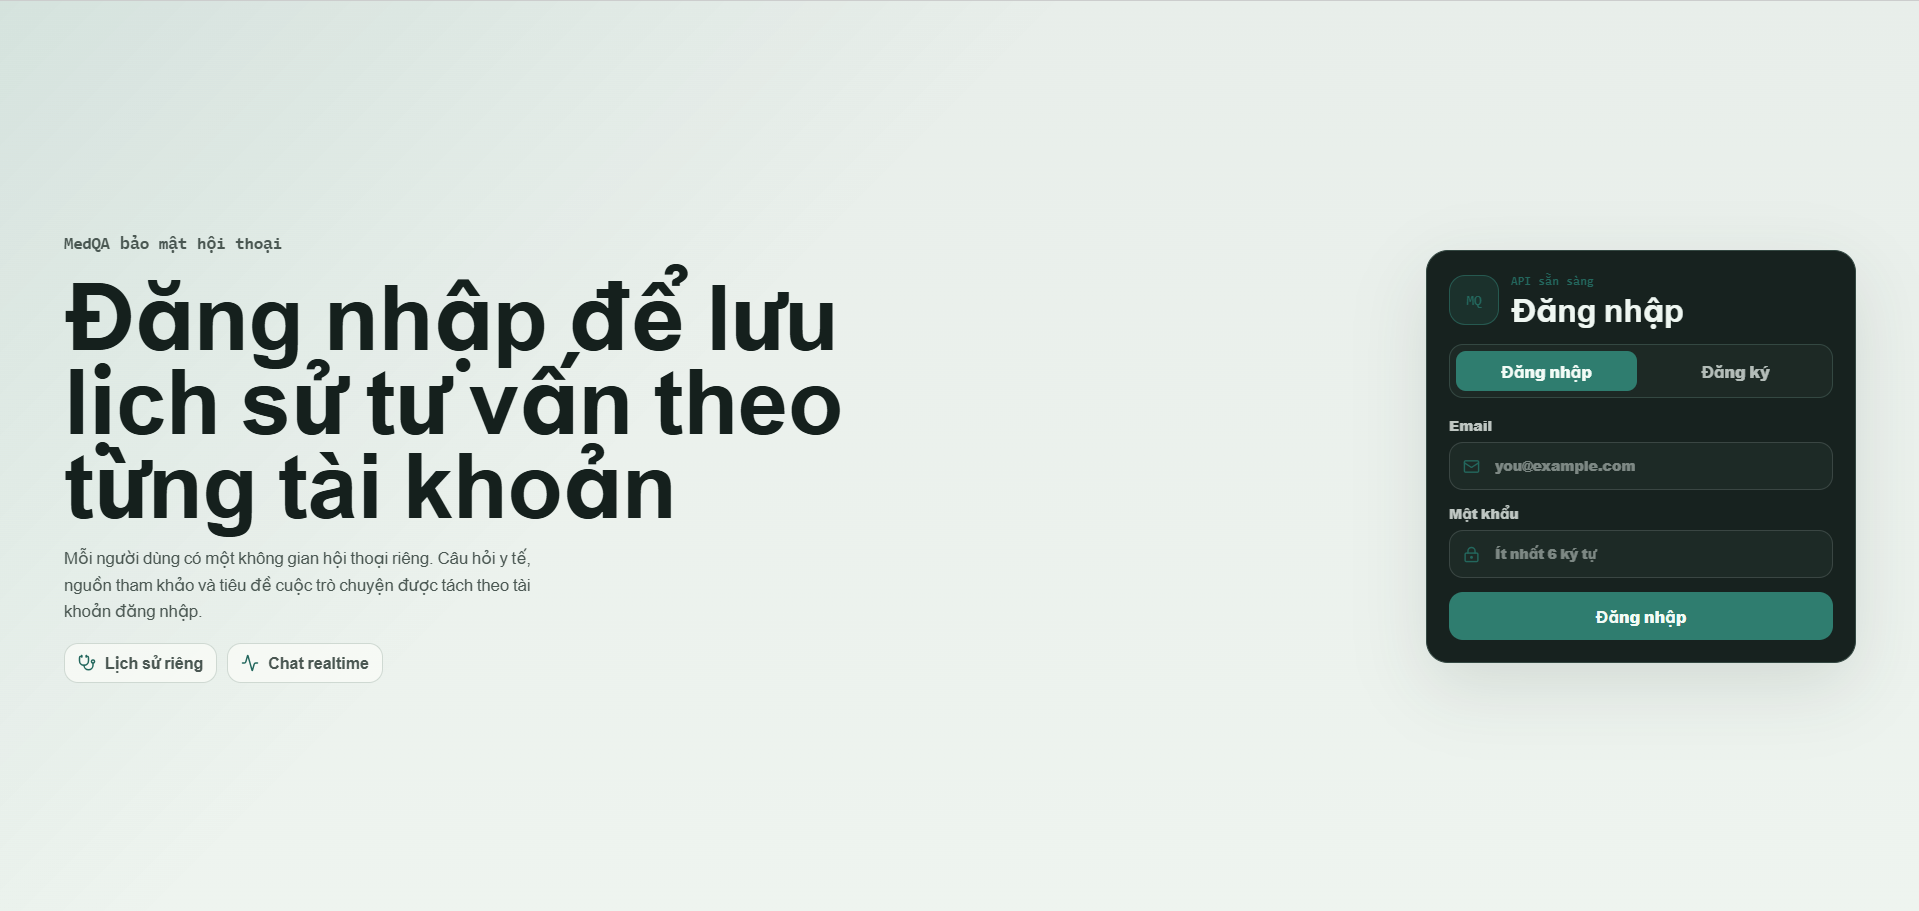
\includegraphics[width=\linewidth]{figures/auth-login-screen.png}
        }{
            \fbox{\parbox[c][3cm][c]{0.95\linewidth}{\centering Chèn ảnh đăng nhập}}
        }
    \end{minipage}
    \hfill
    \begin{minipage}{0.49\textwidth}
        \centering
        \IfFileExists{figures/auth-register-screen.png}{
            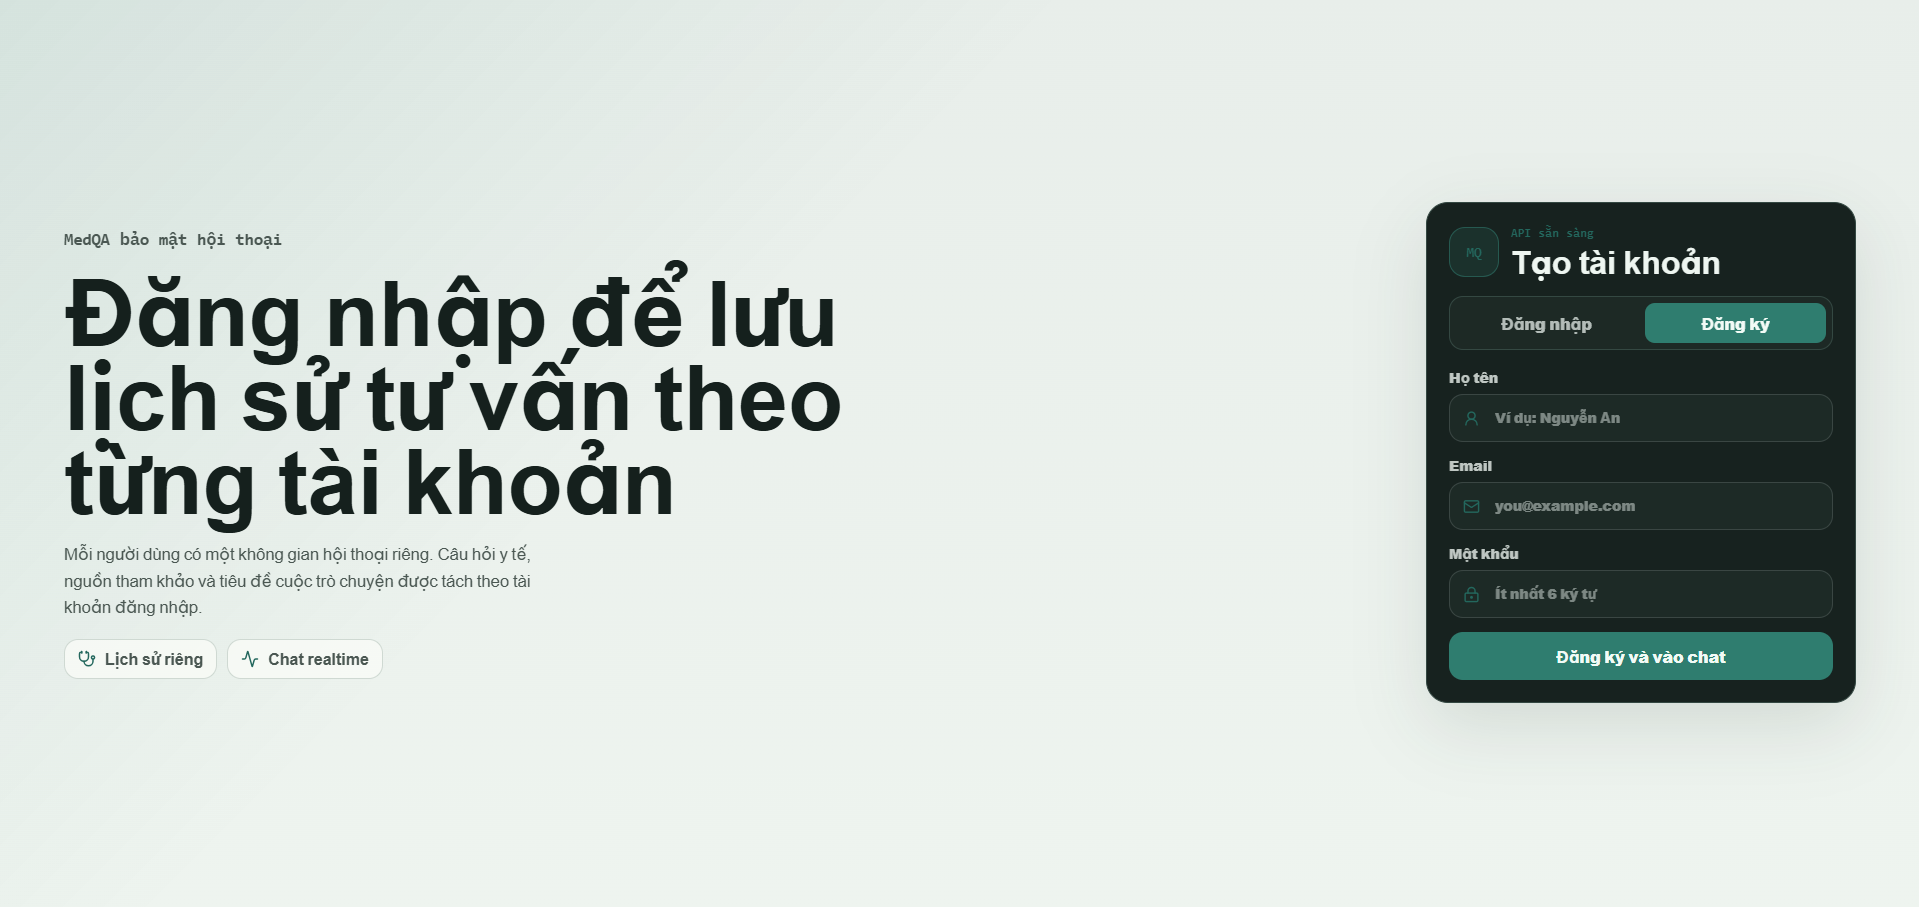
\includegraphics[width=\linewidth]{figures/auth-register-screen.png}
        }{
            \fbox{\parbox[c][3cm][c]{0.95\linewidth}{\centering Chèn ảnh đăng ký}}
        }
    \end{minipage}
    \caption{Màn hình đăng nhập và đăng ký tài khoản.}
    \label{fig:auth-screens}
\end{figure}

\begin{figure}[H]
    \centering
    \IfFileExists{figures/chat-main-screen.png}{
        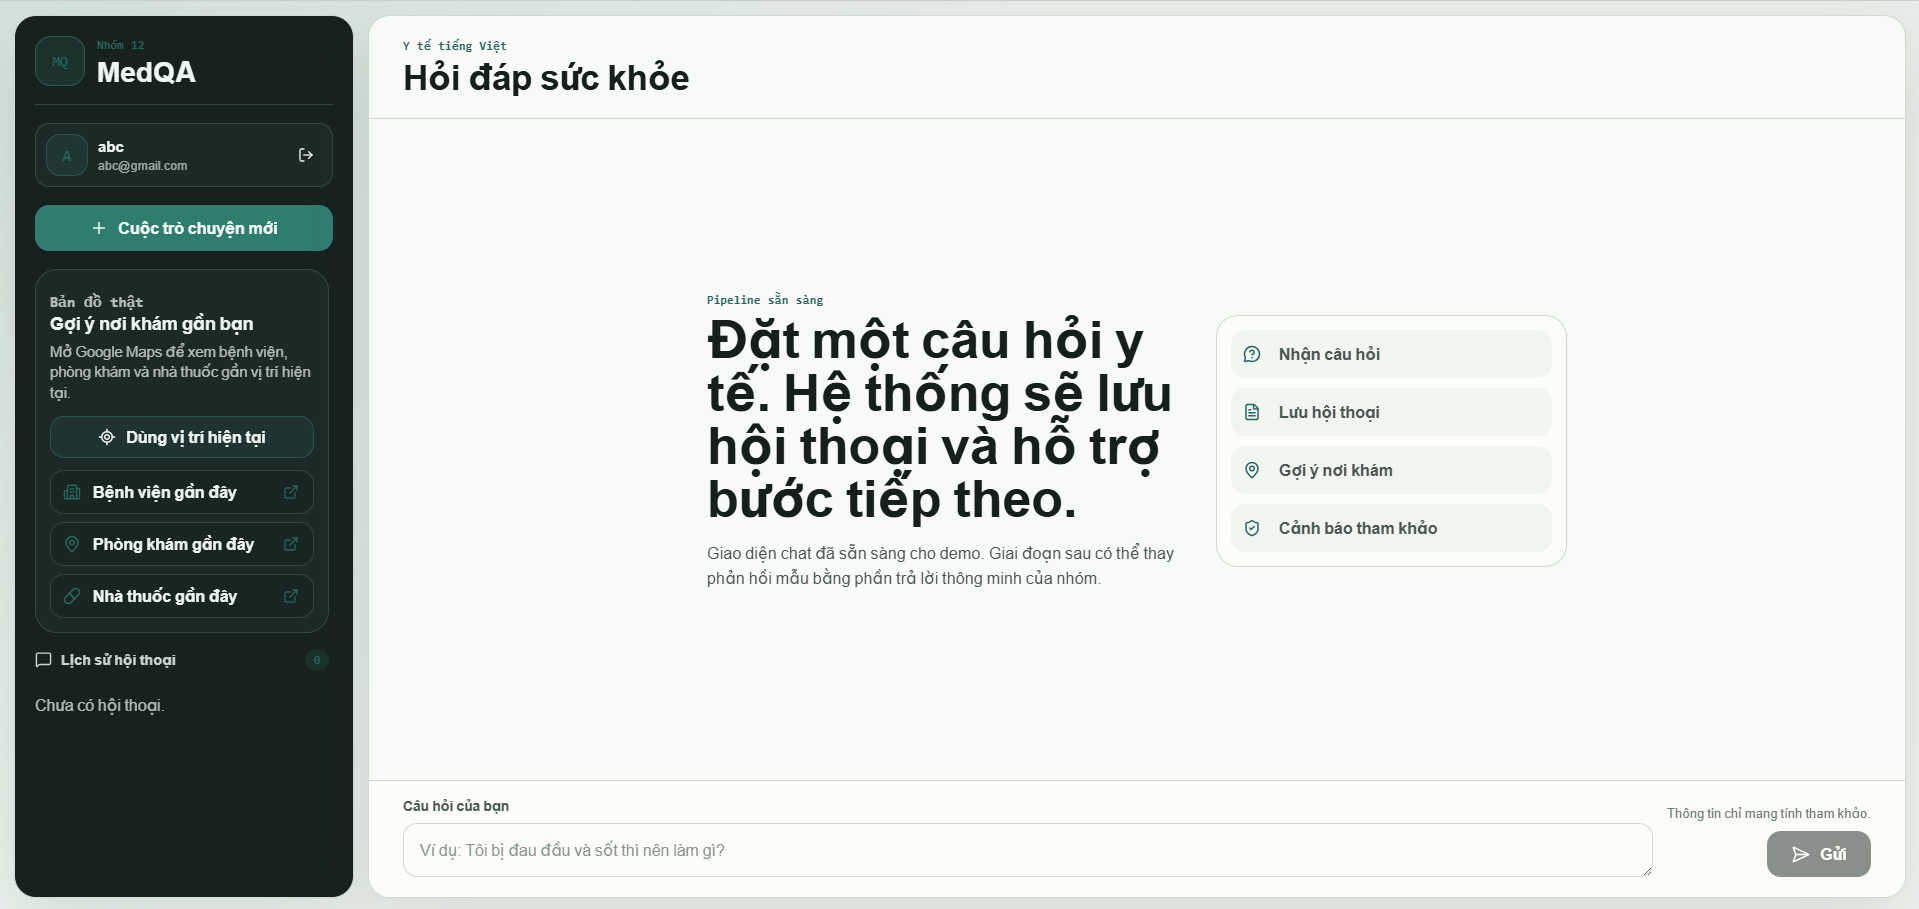
\includegraphics[width=0.86\textwidth]{figures/chat-main-screen.png}
    }{
        \fbox{\parbox[c][4cm][c]{0.86\textwidth}{\centering Chèn ảnh màn hình chatbot}}
    }
    \caption{Giao diện chatbot sau khi đăng nhập.}
    \label{fig:chat-main-screen}
\end{figure}

\begin{figure}[H]
    \centering
    \IfFileExists{figures/nearby-hospitals-screen.png}{
        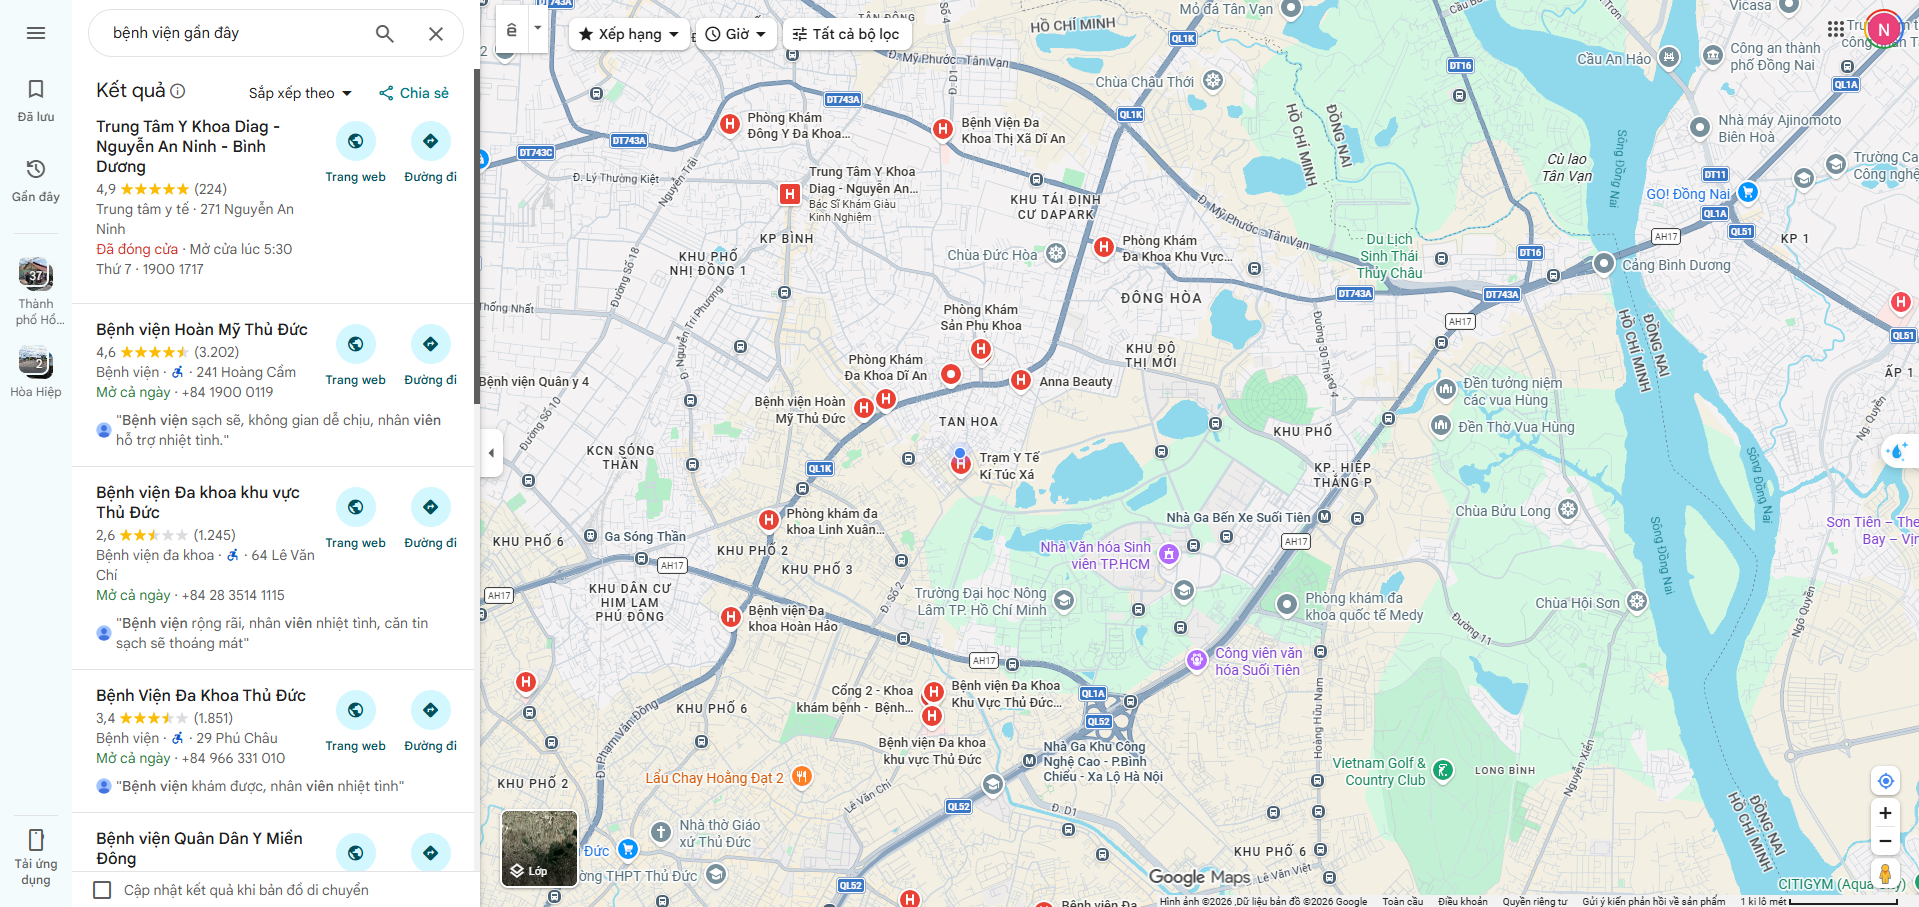
\includegraphics[width=0.86\textwidth]{figures/nearby-hospitals-screen.png}
    }{
        \fbox{\parbox[c][4cm][c]{0.86\textwidth}{\centering Chèn ảnh gợi ý bệnh viện gần đây}}
    }
    \caption{Gợi ý bệnh viện gần đây thông qua Google Maps.}
    \label{fig:nearby-hospitals-screen}
\end{figure}

\section{Triển khai}
Ứng dụng được triển khai trên VPS Ubuntu bằng PM2. Frontend và backend chạy thành hai tiến trình riêng, tránh ảnh hưởng đến các dịch vụ khác trên máy chủ. SQLite được đặt trong thư mục dùng chung để khi cập nhật mã nguồn, dữ liệu người dùng và lịch sử hội thoại không bị mất.

\begin{itemize}
    \item Repository: \url{https://github.com/Nguyennnm/ML-CHATBOT_MEDICAL}
    \item Frontend: \url{http://84.247.147.180:18180}
    \item Backend health check: \url{http://84.247.147.180:18181/api/health}
    \item Database: \texttt{/opt/ml-web/shared/medical\_chatbot.sqlite}
\end{itemize}

Khi chạy local, nhóm cài dependency bằng \texttt{npm install}, chạy migration bằng \texttt{npm run db:migrate} và khởi động frontend/backend bằng \texttt{npm run dev}. Các biến môi trường quan trọng gồm \texttt{PORT}, \texttt{CLIENT\_ORIGIN}, \texttt{DB\_PATH}, \texttt{RAG\_API\_BASE\_URL}, \texttt{AUTH\_TOKEN\_SECRET} và \texttt{AUTH\_TOKEN\_TTL\_SECONDS}.

\section{Kiểm thử và vận hành}
Nhóm đã kiểm thử các luồng chính: đăng ký, đăng nhập, tạo hội thoại, đổi tên, xóa hội thoại, gửi câu hỏi, stream câu trả lời và hiển thị nguồn tham khảo. Với phần phân quyền, hai tài khoản khác nhau được dùng để kiểm tra rằng người dùng không thể xem hoặc truy cập trực tiếp hội thoại của tài khoản khác. API \texttt{/api/conversations} trả \texttt{401} khi thiếu token và trả \texttt{404} khi truy cập hội thoại không thuộc người dùng hiện tại.

Sau khi triển khai, frontend public trả mã \texttt{200}, backend health check trả \texttt{\{"status":"ok"\}}, và hai tiến trình \texttt{ml-web-api}, \texttt{ml-web-client} hoạt động ổn định trên PM2. Ở mức đồ án, hệ thống đã có các biện pháp bảo mật cơ bản như hash mật khẩu, Bearer token, kiểm soát CORS, giới hạn độ dài tin nhắn và tách dữ liệu theo \texttt{user\_id}. Nếu triển khai thực tế, hệ thống nên bổ sung HTTPS, domain, reverse proxy, rate limiting và cơ chế backup cơ sở dữ liệu.

\section{Kết luận chương}
Chương này trình bày phiên bản web của hệ thống hỏi--đáp y tế tiếng Việt. Sản phẩm đã có giao diện React, backend Express MVC, cơ sở dữ liệu SQLite, xác thực người dùng, quản lý lịch sử hội thoại, trả lời realtime bằng SSE, liên kết bản đồ gợi ý cơ sở y tế và triển khai public trên VPS. Đây là nền tảng để nhóm tiếp tục hoàn thiện chất lượng mô hình RAG và mở rộng hệ thống trong các giai đoạn sau.

\chapter{Kết luận}
\label{chap:conclusion}

\section{Tóm tắt kết quả}
Đồ án đã xây dựng được hệ thống hỏi--đáp y tế tiếng Việt theo hướng kết hợp dữ liệu, mô hình học máy và ứng dụng web. Nhóm đã thu thập, làm sạch và phân tích bộ dữ liệu QA y tế; triển khai ba hướng tiếp cận gồm BM25, fine-tuning Qwen2 và RAG; đồng thời so sánh kết quả theo chất lượng trả lời, khả năng bám nguồn và chi phí triển khai. Trong các hướng thử nghiệm, RAG phù hợp nhất với bài toán vì có khả năng truy xuất ngữ cảnh liên quan và trả lời kèm nguồn tham khảo. Bên cạnh phần mô hình, nhóm đã hoàn thiện ứng dụng web gồm React frontend, Express MVC backend, SQLite, đăng nhập/đăng ký, lưu lịch sử hội thoại theo tài khoản, trả lời realtime bằng SSE và gợi ý cơ sở y tế gần người dùng qua Google Maps.

\section{Hạn chế}
Hệ thống vẫn còn một số hạn chế. Dữ liệu y tế tuy có quy mô lớn nhưng chưa được thẩm định đầy đủ bởi chuyên gia, nên có thể chứa nhiễu hoặc thông tin chưa đồng nhất. Việc đánh giá mô hình còn phụ thuộc nhiều vào tập kiểm thử giới hạn và các metric tự động, chưa phản ánh hoàn toàn độ an toàn y khoa của câu trả lời. Mô hình RAG phụ thuộc vào chất lượng truy xuất và dịch vụ inference bên ngoài, vì vậy độ trễ và độ ổn định còn bị ảnh hưởng bởi môi trường chạy. Ứng dụng web hiện phù hợp cho demo học phần; nếu dùng thực tế cần bổ sung HTTPS, kiểm soát truy cập chặt hơn, backup dữ liệu và cơ chế giám sát vận hành.

\section{Hướng phát triển}
Trong tương lai, nhóm có thể mở rộng dữ liệu bằng các nguồn y tế đáng tin cậy hơn và xây dựng tập đánh giá được kiểm tra bởi chuyên gia. Về mô hình, cần cải thiện bước chunking, reranking, lọc nguồn và bổ sung guardrails để giảm nguy cơ trả lời sai hoặc vượt quá phạm vi tư vấn. Về hệ thống, có thể triển khai mô hình trên server ổn định, chuyển SQLite sang PostgreSQL khi số lượng người dùng tăng, thêm domain/HTTPS, logging, rate limiting và cơ chế sao lưu. Các cải tiến này sẽ giúp hệ thống tiến gần hơn tới một chatbot y tế có tính ứng dụng thực tế, an toàn và dễ mở rộng.

% ==================== TÀI LIỆU THAM KHẢO ====================
\printbibliography[heading=bibintoc,title={Tài liệu tham khảo}]



\end{document}

